\mfpicnumber{1}

\opengraphsfile{PowerFunctions}

\setcounter{footnote}{0}

\label{PowerFunctions}

Monomial, and, more generally, Laurent monomial functions  are specific examples of a much larger class of functions called \textbf{power functions}, as defined below.

\colorbox{ResultColor}{\bbm

\begin{defn} \label{powerfunction}  Let $a$ and $p$ be nonzero real numbers.  A  \index{power function}\index{function! power} \textbf{power function} is either a constant function or a  function of the form $f(x) = a x^p$.  

\end{defn}

\ebm}

Definition \ref{powerfunction} broadens our scope of functions to include non-integer exponents such as  $f(x) = 2x^{4/3}$, $g(t) = t^{0.4}$ and  $h(w) = w^{\sqrt{2}}$.   Our primary aim in this section is to ascribe meaning to these quantities.  

\subsection{Rational Number Exponents} 

The road to real number exponents starts by defining rational number exponents. 

\label{RationalExponents}

\smallskip

\colorbox{ResultColor}{\bbm

\begin{defn}  \label{rationalexponentdefna} \index{rational number exponent}\index{exponent, rational number} Let $r$  be a rational number where in lowest terms  $r = \frac{m}{n}$ where $m$ is an integer and $n$ is a natural number.\footnote{Recall `lowest terms' means $m$ and $n$ have no common factors other than $1$.}    If $n = 1$, then $x^{r} = x^{m}$.  If $n > 1$, then  \[ x^{r} = x^{\frac{m}{n}} = \left(\sqrt[n]{x}\right)^m   = \sqrt[n]{x^m}, \] whenever $\left(\sqrt[n]{x} \right)^m$ is defined.\footnote{That is, if $n$ is even, $x \geq 0$ and if $m<0$, $x \neq 0$.}

\end{defn}

\ebm}

\smallskip

There are quite a few items worthy of note which are consequences of Definition \ref{rationalexponentdefna}.  First off, if $m$ is an integer, then $x^{\frac{m}{1}}  = x^{m}$ so expressions like $x^{\frac{3}{1}}$  are synonymous with  $x^3$, as we would expect.\footnote{Either $n=1$ is a special case in Definition \ref{rationalexponentdefna} or we need to define what is meant by $\sqrt[1]{x}$.  The authors chose the former.}   Second, the definition of $x^{\frac{m}{n}}$ can be taken as just $\left(\sqrt[n]{x}\right)^m$ and shown to be equal to $\sqrt[n]{x^m}$ (or vice-versa) courtesy of properties of radicals.  We state both in  Definition \ref{rationalexponentdefna} to allow for the reader to choose whichever form is more convenient in a given situation.  The  critical point to remember is no matter which representation you choose, keep in mind the restrictions if $n$ is even, $x \geq 0$ and if $m < 0$, $x \neq 0$.  

Moreover,  per this definition,  $x^{\frac{1}{n}} = \sqrt[n]{x^{1}} = \sqrt[n]{x}$, so we may rewrite principal roots as exponents: $\sqrt{x} = x^{\frac{1}{2}}$ and $\sqrt[5]{x} = x^{\frac{1}{5}}$. This makes sense from an algebraic standpoint since per Theorem \ref{basicradicalpropseqineq}, $\left(\sqrt[n]{x} \right)^n = x$.  Hence if we were to assign an exponent notation to  $\sqrt[n]{x}$, say $\sqrt[n]{x} = x^r$, then  $\left(\sqrt[n]{x}\right)^n = (x^r)^n = x$.  If the properties of exponents are to hold, then, necessarily, $ (x^r)^n = x^{rn} = x = x^{1}$, so $rn = 1$ or $r = \frac{1}{n}$. While this argument helps \textit{motivate} the notation, as we shall see shortly, great care must be exercised in applying exponent properties in these cases.  The long and short of this is that root functions as defined in Section \ref{RootRadicalFunctions} are all members of the `power functions' family.
  
Another important item worthy of note in Definition \ref {rationalexponentdefna} is that it is absolutely essential  we express the rational number $r$ in \textit{lowest terms} before applying the root-power definition.  For example, consider $x^{0.4}$. Expressing $r$ in lowest terms, we get:  $r = 0.4 = \frac{4}{10} = \frac{2}{5}$.  Hence,  $x^{0.4} = x^{2/5} = (\sqrt[5]{x})^2$ or $\sqrt[5]{x^2}$, either of which is defined for all real numbers $x$.  In contrast, consider the equivalence $r = 0.4 = \frac{4}{10}$.  Here, the expression $(\sqrt[10]{x})^4$ is defined only for $x \geq 0$ owing to the presence of the even indexed root, $\sqrt[10]{x}$.  Hence, $(\sqrt[10]{x})^4 \neq x^{\frac{4}{10}} = x^{\frac{2}{5}}$ unless $x \geq 0$.   On the other hand,  the expression $\sqrt[10]{x^4}$ \textit{is} defined for all numbers, $x$, since $x^4 \geq 0$ for all $x$. In fact,  it can be shown that $\sqrt[10]{x^4} = \sqrt[5]{x^2}$ for all real numbers.  This means  $\sqrt[10]{x^4} =  \sqrt[5]{x^2} = x^{\frac{2}{5}} = x^{\frac{4}{10}}$.   So, to review, in general we have: $x^{\frac{4}{10}} = \sqrt[10]{x^4}$, but $x^{\frac{4}{10}}   \neq \left(\sqrt[10]{x}\right)^{4}$ unless $x \geq 0$.  Once again the easiest way to avoid confusion here is to \textit{reduce} the exponent to \textit{lowest terms} before converting it to root-power notation.


Likewise, we have to be careful about the properties of exponents when it comes to rational exponents.   Consider, for instance, the product rule for integer exponents:  $x^{m} x^{n} = x^{m+n}$.  Consider $f(x) = x^{\frac{1}{2}} x^{\frac{1}{2}}$ and $g(x) = x^{\frac{1}{2} + \frac{1}{2}}$.  In the first case, $f(x) =  x^{\frac{1}{2}} x^{\frac{1}{2}} =\sqrt{x} \sqrt{x} = (\sqrt{x})^2 = x$ only for $x \geq 0$.   In the second case, $g(x) = x^{\frac{1}{2} + \frac{1}{2}} = x^{\frac{2}{2}} = x^{1} = x$ for \text{all} real numbers $x$. Even though $f(x) = g(x)$ for $x \geq 0$, $f$ and $g$ are \textit{different functions} since they have \textit{different domains}.  


Similarly,  the power rule for integer exponents:  $(x^n)^m = x^{nm}$ does not hold  in general for rational exponents. To see this,  consider the three functions: $f(x) = (x^{\frac{1}{2}} )^2$,  $g(x) = x^{\frac{2}{2}}$,  and $h(x) = (x^2)^{\frac{1}{2}}$. In the first case,  $f(x) = (x^{\frac{1}{2}})^2 = (\sqrt{x})^2 = x$ for $x \geq 0$ only (this is the same function $f$ above.)  In the second case,  the rational number $r = \frac{2}{2} = 1$, so $g(x) = x^{\frac{2}{2}} = x^{\frac{1}{1}} = x^{1} = x$ for \textit{all} real numbers, $x$ (this is the same function $g$ from above.)  In the last case,  $h(x) = (x^2)^{\frac{1}{2}} = \sqrt{x^2} = |x|$ for all real numbers, $x$. Once again, despite $f(x) = g(x) = h(x)$ for all $x \geq 0$,  $f$, $g$ and $h$ and are \textit{three different functions}.  We graph $f$, $g$, and $h$ below.  

\begin{multicols}{3}

\begin{mfpic}[15]{-4}{4}{-4}{5}
\axes
\tlabel[cc](4,-0.5){\scriptsize $x$}
\tlabel[cc](0.5,5){\scriptsize $y$}
\point[3pt]{(0,0)}
\xmarks{-3,-2,-1,1,2,3}
\ymarks{-3,-2,-1,1,2,3,4}
\tcaption{\scriptsize $f(x) = x^{\frac{1}{2}} x^{\frac{1}{2}} = (x^{\frac{1}{2}})^2 = x$, $x \geq 0$}
\tlpointsep{4pt}
\axislabels {x}{ {\scriptsize $-3 \hspace{7pt}$} -3, {\scriptsize $-2 \hspace{7pt}$} -2, {\scriptsize $-1 \hspace{7pt}$} -1, {\scriptsize $1$} 1, {\scriptsize $2$} 2, {\scriptsize $3$} 3}
\axislabels {y}{{\scriptsize $-1$} -1, {\scriptsize $-2$} -2, {\scriptsize $-3$} -3,{\scriptsize $1$} 1, {\scriptsize $2$} 2, {\scriptsize $3$} 3, {\scriptsize $4$} 4}
\penwd{1.25pt}
\arrow \polyline{(0,0),(4,4)}
\point[4pt]{(0,0)}
\end{mfpic}

\begin{mfpic}[15]{-4}{4}{-4}{5}
\axes
\tlabel[cc](4,-0.5){\scriptsize $x$}
\tlabel[cc](0.5,5){\scriptsize $y$}
\xmarks{-3,-2,-1,1,2,3}
\xmarks{-3,-2,-1,1,2,3}
\ymarks{-3,-2,-1,1,2,3,4}
\tcaption{\scriptsize $g(x) =  x^{\frac{1}{2} + \frac{1}{2}} = x^{\frac{2}{2}} = x$ }
\tlpointsep{4pt}
\axislabels {x}{ {\scriptsize $-3 \hspace{7pt}$} -3, {\scriptsize $-2 \hspace{7pt}$} -2, {\scriptsize $-1 \hspace{7pt}$} -1, {\scriptsize $1$} 1, {\scriptsize $2$} 2, {\scriptsize $3$} 3}
\axislabels {y}{{\scriptsize $-1$} -1, {\scriptsize $-2$} -2, {\scriptsize $-3$} -3,{\scriptsize $1$} 1, {\scriptsize $2$} 2, {\scriptsize $3$} 3, {\scriptsize $4$} 4}
\penwd{1.25pt}
\arrow \reverse \arrow \polyline{( -4,-4), (4,4)}
\end{mfpic} 



\begin{mfpic}[15]{-4}{4}{-4}{5}
\axes
\tlabel[cc](4,-0.5){\scriptsize $x$}
\tlabel[cc](0.5,5){\scriptsize $y$}
\xmarks{-3,-2,-1,1,2,3}
\xmarks{-3,-2,-1,1,2,3}
\ymarks{-3,-2,-1,1,2,3,4}
\tcaption{\scriptsize $h(x) = (x^2)^{\frac{1}{2}} = |x|$ }
\tlpointsep{4pt}
\axislabels {x}{ {\scriptsize $-3 \hspace{7pt}$} -3, {\scriptsize $-2 \hspace{7pt}$} -2, {\scriptsize $-1 \hspace{7pt}$} -1, {\scriptsize $1$} 1, {\scriptsize $2$} 2, {\scriptsize $3$} 3}
\axislabels {y}{{\scriptsize $-1$} -1, {\scriptsize $-2$} -2, {\scriptsize $-3$} -3,{\scriptsize $1$} 1, {\scriptsize $2$} 2, {\scriptsize $3$} 3, {\scriptsize $4$} 4}
\penwd{1.25pt}
\arrow \reverse \arrow \polyline{(-4,4), (0,0), (4,4)}
\end{mfpic} 

\end{multicols}

In general, the properties of integer exponents \textit{do not extend} to rational exponents \textit{unless} the bases involved represent \text{non-negative} real numbers \textit{or} the roots involved are \textit{odd}.  We have the following:

\colorbox{ResultColor}{\bbm

\begin{thm}  \label{exponentprops} Let $r$ and $s$ are rational numbers.  The following properties hold provided none of the computations results in division by $0$ and \textbf{either}  $r$ and $s$ have odd denominators  \textbf{or}  $x \geq 0$ \textbf{and} $y \geq 0$:

\begin{itemize}

\item \textbf{Product Rules:}  $x^{r} x^{s} = x^{r+s}$ and $(xy)^{r} = x^{r} y^{r}$.

\item \textbf{Quotient Rules:}  $\dfrac{x^{r}}{x^{s}} = x^{r-s}$ and $\left( \dfrac{x}{y}\right)^{r} = \dfrac{x^{r}}{y^{r}}$

\item \textbf{Power Rule:}  $(x^{r})^{s} = x^{rs}$

\end{itemize}

\end{thm}

\ebm}


Next, we turn our attention to the graphs of $f(x) =x^r =  x^{\frac{m}{n}}$ for varying values of $m$ and $n$.  When $n$ is even, the domain is restricted owing to the presence of the even indexed root to $[0, \infty)$. The range is likewise $[0, \infty)$, a fact leave to the reader.  All of the functions below are increasing on their domains, and it turns out this is always the case provided $r>0$.  There is, however, is a difference in \textit{how} the functions are increasing - and this is the concept of \index{concavity}\textit{concavity}.  As with many concepts we've encountered so far in the text,  concavity is most precisely defined using Calculus terminology,  but we can nevertheless get a sense of concavity geometrically.   For us,  a curve is  \index{concave up}\index{concavity ! concave up}\textbf{concave up} over an interval if it resembles a  portion of a `$\smile$' shape.  Similarly, a curve is called  \index{concave down}\index{concavity ! concave down}\textbf{concave down} over an interval if  resembles part of a `$\frown$' shape. When $0 < r < 1$, the graphs of $f(x) = x^r$ resemble the left half of $\frown$ and so are concave down;  when $r>1$, the graphs resemble the right half of a `$\smile$' and are hence described as `concave up.'

\begin{center}

\begin{tabular}{cccc}

\begin{mfpic}[20]{0}{5}{0}{5}
\axes
\tlabel[cc](5, -0.5){\scriptsize $x$}
\tlabel[cc](0.5, 5){\scriptsize $y$}
\tlabel[cc](1,1.75){\scriptsize $(1,1)$}
\tlabel[cc](0,-0.5){\scriptsize $(0,0)$}
\penwd{1.25pt}
\arrow \parafcn{0,2,0.1}{(t^2,t)}
\point[4pt]{(0,0), (1,1)}

\tcaption{\scriptsize $f(x)=x^{\frac{1}{2}}$}
\end{mfpic}

&

\begin{mfpic}[20]{0}{5}{0}{5}
\axes
\tlabel[cc](5, -0.5){\scriptsize $x$}
\tlabel[cc](0.5, 5){\scriptsize $y$}
\tlabel[cc](1,1.75){\scriptsize $(1,1)$}
\tlabel[cc](0,-0.5){\scriptsize $(0,0)$}
\penwd{1.25pt}
\arrow \parafcn{0,1.5,0.1}{(t^4,t^3)}
\point[4pt]{(0,0), (1,1)}
\tcaption{\scriptsize $f(x)=x^{\frac{3}{4}}$}
\end{mfpic}

&


\begin{mfpic}[20]{0}{5}{0}{5}
\axes
\tlabel[cc](5, -0.5){\scriptsize $x$}
\tlabel[cc](0.5, 5){\scriptsize $y$}
\tlabel[cc](1.75,1){\scriptsize $(1,1)$}
\tlabel[cc](0,-0.5){\scriptsize $(0,0)$}
\penwd{1.25pt}
\arrow \parafcn{0,1.35,0.1}{(t**4,t**5)}
\point[4pt]{(0,0), (1,1)}

\tcaption{\scriptsize $f(x)=x^{\frac{5}{4}}$}

\end{mfpic}



&


\begin{mfpic}[20]{0}{5}{0}{5}
\axes
\tlabel[cc](5, -0.5){\scriptsize $x$}
\tlabel[cc](0.5, 5){\scriptsize $y$}
\tlabel[cc](1.75,1){\scriptsize $(1,1)$}
\tlabel[cc](0,-0.5){\scriptsize $(0,0)$}
\penwd{1.25pt}
\arrow \parafcn{0,1.7,0.1}{(t**2,t**3)}
\point[4pt]{(0,0), (1,1)}

\tcaption{\scriptsize $f(x)=x^{\frac{3}{2}}$}

\end{mfpic} \\

\end{tabular}

\end{center}

Below we graph several examples of $f(x) =x^r =  x^{\frac{m}{n}}$ where $n$ is odd.   Here, the domain is $(-\infty, \infty)$ since the index on the root here is odd. Note that when $m$ is even, the graphs appear to be symmetric about the $y$-axis  and the range looks to be $[0, \infty)$.  When $m$ is odd, the graphs  appear to be symmetric about the origin with range $(-\infty, \infty)$.  We leave verification of these facts to the reader.   Note here also that for $x \geq 0$, the graphs are down for $0<r<1$ and concave up for $r > 1$. 

\begin{center}


\begin{tabular}{cccc}

\begin{mfpic}[15]{-4}{4}{-4}{4}
\axes
\tlabel[cc](4, -0.5){\scriptsize $x$}
\tlabel[cc](0.5, 4){\scriptsize $y$}
\tlabel[cc](2,0.75){\scriptsize $(1,1)$}
\tlabel[cc](0.75,-0.5){\scriptsize $(0,0)$}
\tlabel[cc](-2.25,-0.75){\scriptsize $(-1,-1)$}
\penwd{1.25pt}
\arrow \reverse \arrow \parafcn{-1.3,1.3,0.1}{(t^5,t^3)}
\point[4pt]{(0,0), (1,1), (-1,-1)}

\tcaption{\scriptsize $f(x)=x^{\frac{3}{5}}$}
\end{mfpic}

&
\begin{mfpic}[15]{-4}{4}{-4}{4}
\axes
\tlabel[cc](4, -0.5){\scriptsize $x$}
\tlabel[cc](0.5, 4){\scriptsize $y$}
\tlabel[cc](1,1.75){\scriptsize $(1,1)$}
\tlabel[cc](0.75,-0.5){\scriptsize $(0,0)$}
\tlabel[cc](-1,1.75){\scriptsize $(-1,1)$}
\penwd{1.25pt}
\arrow \reverse \arrow \parafcn{-1.587,1.587,0.1}{(t^3,t^2)}
\point[4pt]{(0,0), (1,1), (-1,1)}

\tcaption{\scriptsize $f(x)=x^{\frac{2}{3}}$}
\end{mfpic}


&

\begin{mfpic}[15]{-4}{4}{-4}{4}
\axes
\tlabel[cc](4, -0.5){\scriptsize $x$}
\tlabel[cc](0.5, 4){\scriptsize $y$}
\tlabel[cc](1.75,1){\scriptsize $(1,1)$}
\tlabel[cc](0.75,-0.5){\scriptsize $(0,0)$}
\tlabel[cc](-2.25,1){\scriptsize $(-1,1)$}
\penwd{1.25pt}
\arrow \reverse \arrow \parafcn{-1.16,1.16,0.1}{(t^5,t^8)}
\point[4pt]{(0,0), (1,1), (-1,1)}
\tcaption{\scriptsize $f(x)=x^{\frac{8}{5}}$}
\end{mfpic}


&

\begin{mfpic}[15]{-4}{4}{-4}{4}
\axes
\tlabel[cc](4, -0.5){\scriptsize $x$}
\tlabel[cc](0.5, 4){\scriptsize $y$}
\tlabel[cc](1.75,1){\scriptsize $(1,1)$}
\tlabel[cc](0.75,-0.5){\scriptsize $(0,0)$}
\tlabel[cc](-2.25,-1){\scriptsize $(-1,-1)$}
\penwd{1.25pt}
\arrow \reverse \arrow \parafcn{-1.3,1.3,0.1}{(t^3,t^5)}
\point[4pt]{(0,0), (1,1), (-1,-1)}
\tcaption{\scriptsize $f(x)=x^{\frac{5}{3}}$}

\end{mfpic}

\end{tabular}

\end{center}

When $r<0$, we have variables appear in the denominator which open the opportunities for vertical and horizontal asymptotes. Below are graphed two examples

\begin{center}

\begin{tabular}{m{2.5in}m{2.5in}}

\begin{mfpic}[20]{0}{5}{0}{3}
\axes
\tlabel[cc](5, -0.5){\scriptsize $x$}
\tlabel[cc](0.5, 3){\scriptsize $y$}
\tlabel[cc](-1.25,2.5){\scriptsize VA $x =0$}

\tlabel[cc](2.5, -0.5){\scriptsize HA $y =0$}

\tlabel[cc](1.5,1.5){\scriptsize $(1,1)$}
\penwd{1.25pt}
\arrow \reverse \arrow \parafcn{0.45,2.5,0.1}{(1/(t**2),t)}
\point[4pt]{(1,1)}
\tcaption{\scriptsize $f(x)=x^{-\frac{1}{2}}$}

\end{mfpic}

&

\begin{mfpic}[15]{-4}{4}{-4}{4}
\axes
\tlabel[cc](4, -0.5){\scriptsize $x$}
\tlabel[cc](0.5, 4){\scriptsize $y$}
\tlabel[cc](-1.25,2.5){\scriptsize VA $x =0$}
\tlabel[cc](2.5, -0.5){\scriptsize HA $y =0$}
\tlabel[cc](1.75,1){\scriptsize $(1,1)$}
\tlabel[cc](-2.25,-1){\scriptsize $(-1,-1)$}
\penwd{1.25pt}
 \arrow \reverse \arrow \parafcn{-2, -0.65,0.1}{(t,1/t**3)}
\arrow  \reverse \arrow \parafcn{0.65,2,0.1}{(t,1/t**3)}
\point[4pt]{(1,1), (-1,-1)}

\tcaption{\scriptsize $f(x)=x^{-\frac{1}{3}}$}

\end{mfpic}

\\

\end{tabular}

\end{center}


Unsurprisingly, Theorem \ref{linearrootgraphs}, which, as stated, applied to root functions, generalizes to all rational powers.  

\smallskip


\colorbox{ResultColor}{\bbm

\begin{thm} \label{linearrationalpowergraphs}  For real numbers $a$, $b$, $h$, and $k$ and rational number $r$ with $a, b, r \neq 0$, the graph of $F(x) = a(bx-h)^r +k$  can be obtained from the graph of $f(x) = x^r$ by performing the following operations, in sequence:

\begin{enumerate}

\item  add $h$ to each of the $x$-coordinates of the points on the graph of $f$.  This results in a horizontal shift to the right if $h > 0$ or left if $h < 0$.

\textbf{NOTE:}  This transforms the graph of $y =x^{r}$ to $y = (x-h)^{r}$.

\item  divide the $x$-coordinates of the points on the graph obtained in Step 1 by $b$.  This results in a horizontal scaling, but may also include a reflection about the $y$-axis if $b < 0$.

\textbf{NOTE:}  This transforms the graph of $y = (x-h)^{r}$ to $y = (bx-h)^{r}$.

\item  multiply the $y$-coordinates of the points on the graph obtained in Step 2 by $a$.   This results in a vertical scaling, but may also include a reflection about the $x$-axis if $a < 0$.

\textbf{NOTE:}  This transforms the graph of $y = (bx-h)^{r}$ to $y = a(bx-h)^{r}$.

\item  add $k$ to each of the $y$-coordinates of the points on the graph obtained in Step 3.  This results in a vertical shift up if $k > 0$ or down if $k< 0$.

\textbf{NOTE:}  This transforms the graph of $y = a(bx-h)^{r}$ to $y = a(bx-h)^{r}+k$.

\end{enumerate}

\end{thm}

\ebm}

\smallskip

The proof of Theorem \ref{linearrationalpowergraphs} is identical to that of Theorem \ref{linearrootgraphs}, and we suggest the reader work through the details.  We give Theorem \ref{linearrationalpowergraphs}  a test run in the following example.

\begin{ex} \label{rationalpowershiftex} Use the given graphs of $f$ and $g$ below long with Theorem \ref{linearrationalpowergraphs} to graph $F$ and $G$.  State the domain and range of $F$ and $G$ using interval notation.

\begin{enumerate}

\begin{multicols}{2}

\item Graph $F(x) = (2x-1)^{2.6}$.

\item  Graph $G(t) = 1 - 2(t+3)^{\frac{3}{8}}$.

\end{multicols}

\end{enumerate}

\begin{center}

\begin{tabular}{m{2.5in}m{2.5in}}

\begin{mfpic}[20]{-3}{3}{-4}{4}
\axes
\tlabel[cc](3, -0.5){\scriptsize $x$}
\tlabel[cc](0.5, 4){\scriptsize $y$}
\tlabel[cc](1.5,1){\scriptsize $(1,1)$}
\tlabel[cc](-2,-1){\scriptsize $(-1,-1)$}
\tlabel[cc](0.5,-0.5){\scriptsize $(0,0)$}
\penwd{1.25pt}
\arrow \reverse \arrow \parafcn{-1.11, 1.11,0.1}{(t**5,t**13)}

\point[4pt]{(-1,-1), (0,0), (1,1)}
\tcaption{\scriptsize $f(x)=x^{2.6}$}

\end{mfpic}

&

\begin{mfpic}[20]{-1}{5}{-1}{4}
\axes
\tlabel[cc](5, -0.5){\scriptsize $t$}
\tlabel[cc](0.5, 4){\scriptsize $y$}
\tlabel[cc](1,1.5){\scriptsize $(1,1)$}
\tlabel[cc](0.5,-0.5){\scriptsize $(0,0)$}
\penwd{1.25pt}
\arrow  \parafcn{0, 1.22,0.1}{(t**8,t**3)}
\point[4pt]{(0,0), (1,1)}
\tcaption{\scriptsize $g(t)=t^{\frac{3}{8}}$}

\end{mfpic} \\

\end{tabular}

\end{center}


{\bf Solution.}

\begin{enumerate}

\item  The expression  $F(x) = (2x-1)^{2.6}$ is given to us in the form prescribed by Theorem \ref{linearrationalpowergraphs}, and we identify $r = 2.6$, $a = 1$, $b=2$, $h=1$, and $k=0$.  Even though the graph of $f(x) = x^{2.6}$ is given to us, it's worth taking a moment to reinforce some concepts.  Since, in lowest terms, $2.6 = \frac{26}{10} = \frac{13}{5}$, it makes sense the domain and range of $f(x) = x^{2.6}$ are both all real numbers and the graph is symmetric about the origin.\footnote{The domain is all real numbers since the denominator (root) $5$ is odd;  the range is all real numbers since the numerator (power) $13$ is odd.  Since both power and root are odd, the function itself is an odd function, hence the symmetry about the origin.} Moreover, since $2.6>1$, the concavity matches what we would expect, too.  We proceed as we have several times in the past, beginning with the horizontal shift.

Step 1:   add $1$ to each of the $x$-coordinates of each of the points on the graph of $y=x^{2.6}$:

\[ \begin{array}[v]{rlc}


\begin{mfpic}[20]{-3}{3}{-4}{4}
\axes
\tlabel[cc](3, -0.5){\scriptsize $x$}
\tlabel[cc](0.5, 4){\scriptsize $y$}
\tlabel[cc](1.5,1){\scriptsize $(1,1)$}
\tlabel[cc](-2,-1){\scriptsize $(-1,-1)$}
\tlabel[cc](0.5,-0.5){\scriptsize $(0,0)$}
\penwd{1.25pt}
\arrow \reverse \arrow \parafcn{-1.11, 1.11,0.1}{(t**5,t**13)}

\point[4pt]{(-1,-1), (0,0), (1,1)}
\tcaption{\scriptsize $y=x^{2.6}$}

\end{mfpic}
&
\stackrel{\text{ \scriptsize add $1$ to each $x$-coordinate}}{\xrightarrow{\hspace{1.5in}}}
&

\begin{mfpic}[20]{-2}{4}{-4}{4}
\axes
\tlabel[cc](4, -0.5){\scriptsize $x$}
\tlabel[cc](0.5, 4){\scriptsize $y$}
\tlabel[cc](2.5,1){\scriptsize $(2,1)$}
\tlabel[cc](-1,-1){\scriptsize $(0,-1)$}
\tlabel[cc](1.5,-0.5){\scriptsize $(1,0)$}
\penwd{1.25pt}
\arrow \reverse \arrow \parafcn{-1.11, 1.11,0.1}{(t**5+1,t**13)}

\point[4pt]{(0,-1), (1,0), (2,1)}
\tcaption{\scriptsize $y=(x-1)^{2.6}$}

\end{mfpic}\\

 \text{\scriptsize  $(-1,1)$, $(0,0)$, $(1,1)$} & & \text{\scriptsize  $(0,-1)$, $(1,0)$, $(2,1)$} \\
 
 \end{array} \]

Step 2:   divide each of the $x$-coordinates of each of the points on the graph of $y=(x-1)^{2.6}$ by $2$:

\[ \begin{array}[v]{rlc}

\begin{mfpic}[20]{-2}{4}{-4}{4}
\axes
\tlabel[cc](4, -0.5){\scriptsize $x$}
\tlabel[cc](0.5, 4){\scriptsize $y$}
\tlabel[cc](2.5,1){\scriptsize $(2,1)$}
\tlabel[cc](-1,-1){\scriptsize $(0,-1)$}
\tlabel[cc](1.5,-0.5){\scriptsize $(1,0)$}
\penwd{1.25pt}
\arrow \reverse \arrow \parafcn{-1.11, 1.11,0.1}{(t**5+1,t**13)}

\point[4pt]{(0,-1), (1,0), (2,1)}
\tcaption{\scriptsize $y=(x-1)^{2.6}$}

\end{mfpic}
&
\stackrel{\text{ \scriptsize divide to each $x$-coordinate by 2}}{\xrightarrow{\hspace{1.5in}}}
&
\begin{mfpic}[20]{-2}{4}{-4}{4}
\axes
\tlabel[cc](4, -0.5){\scriptsize $x$}
\tlabel[cc](0.5, 4){\scriptsize $y$}
\tlabel[cc](1.5,1){\scriptsize $(1,1)$}
\tlabel[cc](-1,-1){\scriptsize $(0,-1)$}
\tlabel[cc](1,-0.5){\scriptsize $\left(\frac{1}{2},0 \right)$}
\penwd{1.25pt}
\arrow \reverse \arrow \parafcn{-1.11, 1.11,0.1}{((t**5+1)/2,t**13)}

\point[4pt]{(0,-1), (0.5,0), (1,1)}
\tcaption{\scriptsize $F(x)=(2x-1)^{2.6}$}

\end{mfpic}  \\

 \text{\scriptsize   $(0,-1)$, $(1,0)$, $(2,1)$} & & \text{\scriptsize  $(0,-1)$, $\left(\frac{1}{2},0 \right)$, $(1,1)$} \\
 
 \end{array} \]
 
 We get the domain and range here are both $(-\infty, \infty)$.
 
 \item We first need to rewrite $G(t) = 1 - 2(t+3)^{\frac{3}{8}}$ in the form required by Theorem \ref{linearrationalpowergraphs}:  $G(t) =- 2(t+3)^{\frac{3}{8}} + 1$.  We identify $r = \frac{3}{8}$, $a = -2$, $b = 1$, $h = -3$, and $k = 1$.  Since $\frac{3}{8}$ is in lowest terms and has an even denominator,  it makes sense the domain and range of $g(t) = t^{\frac{3}{8}}$ is $[0, \infty)$, since the root here, $8$ is even.  Also, since $0< \frac{3}{8} < 1$, the graph of  $y = t^{\frac{3}{8}}$ is concave down, as we would expect. As usual, we start with the horizontal shift.
 
Step 1:   add $-3$ to each of the $t$-coordinates of each of the points on the graph of $y=t^{\frac{3}{8}}$:

\[ \begin{array}[v]{rlc}

\begin{mfpic}[20]{-1}{5}{-1}{4}
\axes
\tlabel[cc](5, -0.5){\scriptsize $t$}
\tlabel[cc](0.5, 4){\scriptsize $y$}
\tlabel[cc](1,1.5){\scriptsize $(1,1)$}
\tlabel[cc](0.5,-0.5){\scriptsize $(0,0)$}
\penwd{1.25pt}
\arrow  \parafcn{0, 1.22,0.1}{(t**8,t**3)}
\point[4pt]{(0,0), (1,1)}
\tcaption{\scriptsize $y=t^{\frac{3}{8}}$}

\end{mfpic} 


&
\stackrel{\text{ \scriptsize add $-3$ to each $t$-coordinate}}{\xrightarrow{\hspace{1.5in}}}
&

\begin{mfpic}[20]{-4}{2}{-1}{4}
\axes
\tlabel[cc](2, -0.5){\scriptsize $t$}
\tlabel[cc](0.5, 4){\scriptsize $y$}
\tlabel[cc](-2,1.5){\scriptsize $(-2,1)$}
\tlabel[cc](-3,-0.5){\scriptsize $(-3,0)$}
\penwd{1.25pt}
\arrow  \parafcn{0, 1.22,0.1}{(t**8-3,t**3)}
\point[4pt]{(-3,0), (-2,1)}
\tcaption{\scriptsize $y=(t+3)^{\frac{3}{8}}$}

\end{mfpic}   \\

 \text{\scriptsize  $(0,0)$, $(1,1)$} & & \text{\scriptsize  $(-3,0)$, $(-2,1)$} \\
 
 \end{array} \]

 Step 2:  Since $b=1$, we proceed directly to Step 3.
 
 Step 3:   multiply each of the $y$-coordinates of each of the points on the graph of $y=(t+3)^{\frac{3}{8}}$ by $-2$:

\[ \begin{array}[v]{rlc}

\begin{mfpic}[20]{-4}{2}{-1}{4}
\axes
\tlabel[cc](2, -0.5){\scriptsize $t$}
\tlabel[cc](0.5, 4){\scriptsize $y$}
\tlabel[cc](-2,1.5){\scriptsize $(-2,1)$}
\tlabel[cc](-3,-0.5){\scriptsize $(-3,0)$}
\penwd{1.25pt}
\arrow  \parafcn{0, 1.22,0.1}{(t**8-3,t**3)}
\point[4pt]{(-3,0), (-2,1)}
\tcaption{\scriptsize $y=(t+3)^{\frac{3}{8}}$}

\end{mfpic}


&
\stackrel{\text{ \scriptsize multiply each $y$-coordinate by $-2$}}{\xrightarrow{\hspace{1.5in}}}
&

\begin{mfpic}[20]{-4}{2}{-4}{1}
\axes
\tlabel[cc](2, -0.5){\scriptsize $t$}
\tlabel[cc](0.5, 1){\scriptsize $y$}
\tlabel[cc](-2,-3){\scriptsize $(-2,-2)$}
\tlabel[cc](-3,0.5){\scriptsize $(-3,0)$}
\penwd{1.25pt}
\arrow  \parafcn{0, 1.22,0.1}{(t**8-3,(-2)*(t**3))}
\point[4pt]{(-3,0), (-2,-2)}
\tcaption{\scriptsize $y=-2(t+3)^{\frac{3}{8}}$}

\end{mfpic} \\

 \text{\scriptsize  $(-3,0)$, $(-2,1)$} & & \text{\scriptsize  $(-3,0)$, $(-2,-2)$} \\
 
 \end{array} \]
 
 
  Step 4:   add $1$ to each of the $y$-coordinates of each of the points on the graph of $y=-2(t+3)^{\frac{3}{8}}$:

\[ \begin{array}[v]{rlc}

\begin{mfpic}[20]{-4}{2}{-4}{1}
\axes
\tlabel[cc](2, -0.5){\scriptsize $t$}
\tlabel[cc](0.5, 1){\scriptsize $y$}
\tlabel[cc](-2,-3){\scriptsize $(-2,-2)$}
\tlabel[cc](-3,0.5){\scriptsize $(-3,0)$}
\penwd{1.25pt}
\arrow  \parafcn{0, 1.22,0.1}{(t**8-3,(-2)*(t**3))}
\point[4pt]{(-3,0), (-2,-2)}
\tcaption{\scriptsize $y=-2(t+3)^{\frac{3}{8}}$}

\end{mfpic}


&
\stackrel{\text{ \scriptsize add $1$ to each  $y$-coordinate}}{\xrightarrow{\hspace{1.5in}}}
&

\begin{mfpic}[20]{-4}{2}{-3}{2}
\axes
\tlabel[cc](2, -0.5){\scriptsize $t$}
\tlabel[cc](0.5, 2){\scriptsize $y$}
\tlabel[cc](-2,-2){\scriptsize $(-2,-1)$}
\tlabel[cc](-3,1.5){\scriptsize $(-3,1)$}
\penwd{1.25pt}
\arrow  \parafcn{0, 1.22,0.1}{(t**8-3,(-2)*(t**3)+1)}
\point[4pt]{(-3,1), (-2,-1)}
\tcaption{\scriptsize $y=-2(t+3)^{\frac{3}{8}}+1$}

\end{mfpic} \\

 \text{\scriptsize  $(-3,0)$, $(-2,-2)$} & & \text{\scriptsize  $(-3,1)$, $(-2,-1)$} \\
 
 \end{array} \]

From the graph, we get the domain is $[-3, \infty)$ and the range is $(-\infty, 1]$.

\end{enumerate}

\end{ex}

We now turn our attention to more complicated functions involving rational exponents.


\begin{ex}  For the following functions:

\begin{itemize}

\item Analytically:

\begin{multicols}{3}

\begin{itemize}

\item find the domain.

\item find the axis intercepts.

\item analyze the end behavior.

\end{itemize}

\end{multicols}


\item Graph the function with help from a graphing utility and determine:

\begin{multicols}{2}

\begin{itemize}

\item  the range.

\item the local extrema, if they exist.

\end{itemize}

\end{multicols}

\begin{multicols}{2}

\begin{itemize}

\item intervals of increase.

\item intervals of decrease.

\end{itemize}

\end{multicols}

\item Construct a sign diagram for each function using the intercepts and graph.
\end{itemize}

\begin{multicols}{2}
\begin{enumerate}

\item  $f(x) = 3x^2(x^3-8)^{-\frac{2}{3}}$ \vphantom{, $g(t) = \dfrac{(x^2-4)^{\frac{3}{2}}}{x^2-36}$}

\item  $g(t) = \dfrac{(t^2-4)^{\frac{3}{2}}}{t^2-36}$

\end{enumerate}
\end{multicols}

{\bf Solution.}

\begin{enumerate}

\item We first note that, owing to the negative exponent, the quantity $(x^3-8)^{\frac{2}{3}}$ is in the denominator, alerting us to a potential domain issue.  Rewriting $(x^3-8)^{\frac{2}{3}}$ we set about solving $\sqrt[3]{(x^3-8)^2} = 0$.  Cubing both sides and extracting square roots gives $x^3-8=0$ or $x =2$.   Hence, $x =2$ is excluded from the domain.\footnote{In general if $u^{p} = 0$ where $p>0$, then $u =0$.}   Since the root involved here is odd ($3$), the only issue we have is with the denominator, hence our domain is $\{ x \in \mathbb{R} \, | \, x \neq 2 \}$ or $(-\infty, 2) \cup (2, \infty)$.  

While not required to do so, we analyze the behavior of $f$ near $x = 2$.  As $x \rightarrow 2^{-}$, $3x^2 \approx 12$ and $x^3-8 \approx \text{small $(-)$}$.  Hence, $(x^3-8)^{\frac{2}{3}} =\sqrt[3]{(x^3-8)^2} \approx \sqrt[3]{(\text{small $(-)$})^2} \approx \sqrt[3]{\text{small $(+)$}} \approx \text{small$(+)$}$.  As such,  $f(x) \approx \frac{12}{ \text{small$(+)$}} \approx \text{big $(+)$}$.  We conclude as $x \rightarrow 2^{-}$, $f(x) \rightarrow \infty$. As $x \rightarrow 2^{+}$, $3x^2 \approx 12$ and $x^3 - 8 \approx \text{small $(+)$}$, and we likewise get $f(x) \rightarrow \infty$.  This analysis suggests $x=2$ is a vertical asymptote to the graph.


To find the $x$-intercepts, we set $f(x) =  3x^2(x^3-8)^{-\frac{2}{3}} = 0$, so that $3x^2 = 0$ or $x = 0$.  We get $(0,0)$ is our only $x$- (and $y$-)intercept.  

For end behavior, we note that in the denominator the $x^3$ term dominates the constant term, so as $x \rightarrow \pm \infty$, \[ f(x) = 3x^2(x^3-8)^{-\frac{2}{3}} = \dfrac{3x^2}{(x^3-8)^{\frac{2}{3}}} \approx \dfrac{3x^2}{ (x^3)^{ \frac{2}{3} } } = \dfrac{3x^2}{\sqrt[3]{(x^3)^2}} = \dfrac{3x^2}{\sqrt[3]{x^6}} = \dfrac{3x^2}{x^2} = 3.\]  This suggests $y = 3$ is a horizontal asymptote to the graph.

Graphing $y=f(x)$ below on the right bears out our analysis regarding zeros and asymptotes.  The range appears to be $[0, \infty)$, with the graph of $y = f(x)$ crossing its horizontal asymptote between $x=1$ and $x=2$.    We see we have  a single local minimum at $(0,0)$ with $f$ is decreasing on $(-\infty, 0]$ and $(2, \infty)$ and increasing on $[0, 2)$.  

For the  sign diagram, we note that $f$ has only one zero, $x=0$ and is undefined at $x = 2$.  For all $x$ values between these two numbers, $f(x) > 0$ or $(+)$.  Our  sign diagram for $f(x)$ is below on the right.

\begin{center}

\begin{tabular}{cc}

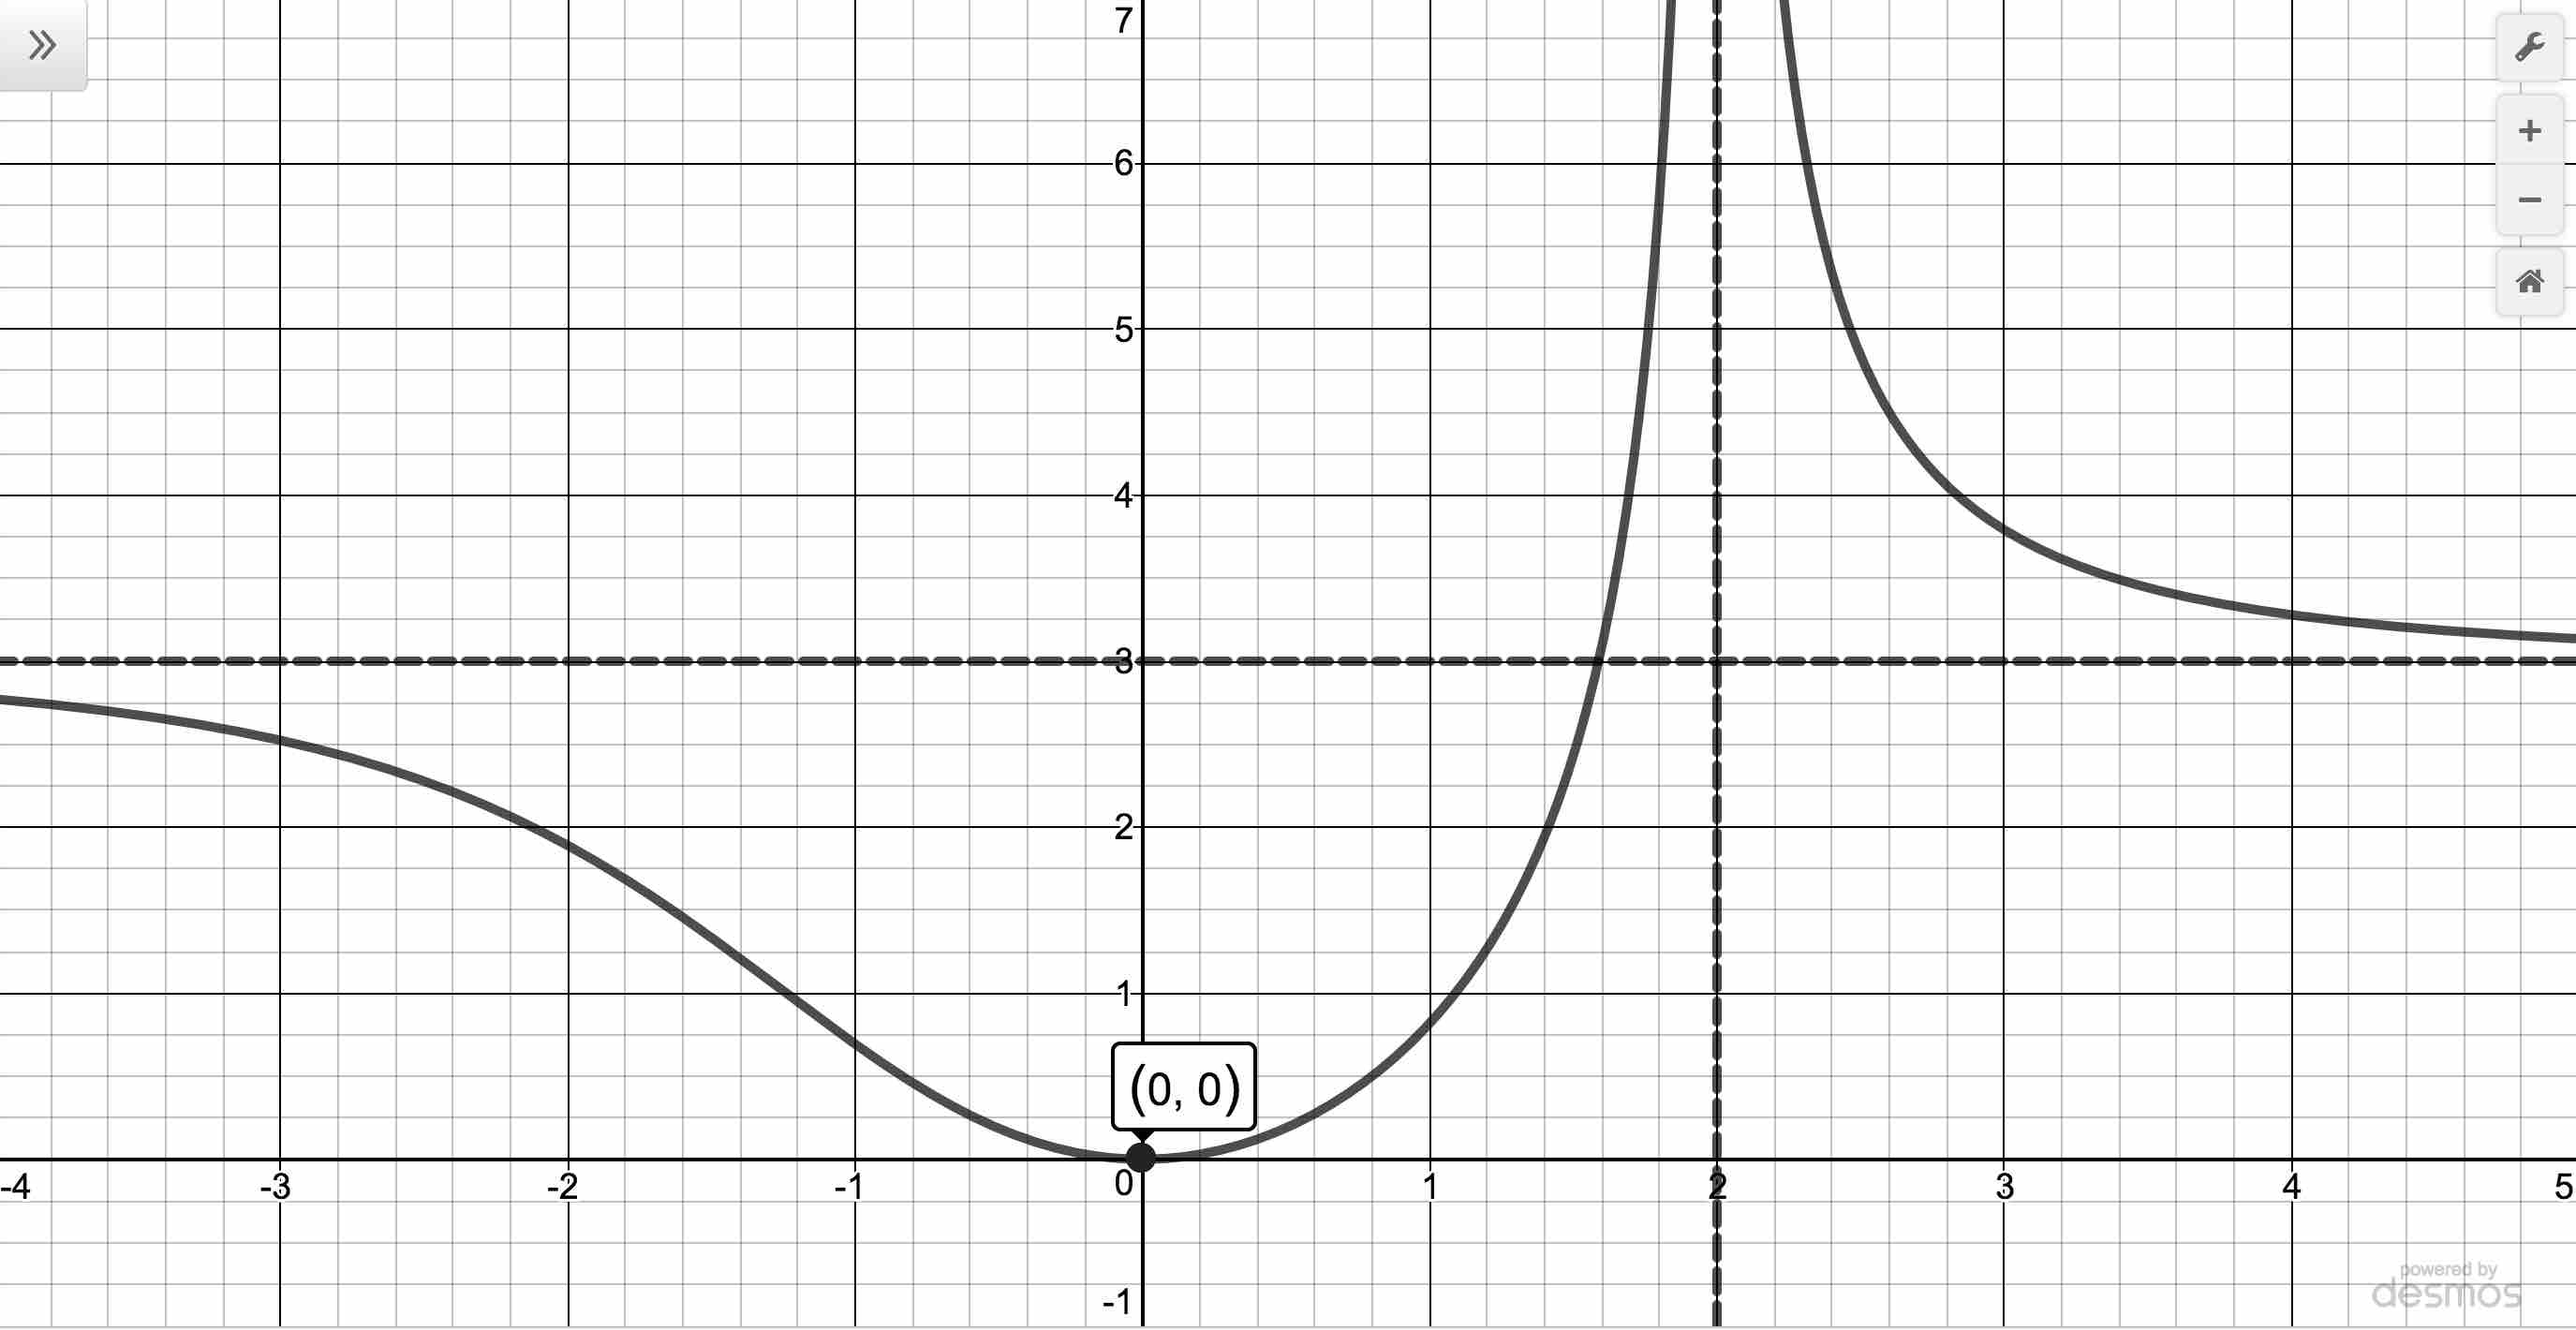
\includegraphics[width=3in]{./PowerFunctionsGraphics/RationalExpEx01.jpg} &

\begin{mfpic}[20]{-4}{2}{-1}{1}
\arrow \reverse \arrow \polyline{(-4,0),(2,0)}
\xmarks{-2,0}
\tlabel[cc](-3, 0.5){$(+)$}
\tlabel[cc](-2,-0.5){$0$}
\tlabel[cc](-2,0.5){$0$}
\tlabel[cc](-1,0.5){$(+)$}
\tlabel[cc](0,-0.5){$2$}
\tlabel[cc](0,0.5){\textinterrobang}
\tlabel[cc](1,0.5){$(+)$}
\end{mfpic}  \\

The graph of $y=f(x)$  \hspace{0.75in} & Sign Diagram for $f(x)$ \\

\end{tabular}

\end{center} 


\item To find the domain of $g(t) = \frac{ (t^2-4)^{\frac{3}{2}} }{t^2-36}$, we have two issues to address:  the denominator and an even (square) root.  Solving $t^2 - 36 = 0$ gives  two excluded values, $t = \pm 6$.  For the numerator, we may rewrite $(t^2-4)^{\frac{3}{2}} = (\sqrt{t^2-4})^3$, so we require $t^2-4 \geq 0$, or  $t^2 \geq 4$.  Extracting square roots, we have $\sqrt{t^2} \geq \sqrt{4}$ or $|t| \geq 2$ which means $t \leq -2$ or $t \geq 2$.  Taking into account our excluded values $t = \pm 6$, we get  the domain of $g$ is $(-\infty, -6) \cup (-6, -2] \cup [2, 6) \cup (6, \infty)$.

Looking near $t = -6$, we note that as $t \rightarrow -6$, $(t^2-4)^{\frac{3}{2}} \approx 32^{\frac{3}{2}} = 32^{1.5}$, a positive number.  As $t \rightarrow -6^{-}$, $t^2-36 \approx \text{small $(+)$}$, so $g(t) \approx \frac{32^{1.5}}{\text{small$(+)$}} \approx \text{big $(+)$}$.  This suggests as $t \rightarrow -6^{-}$, $g(t) \rightarrow \infty$.  On the other hand, as $t \rightarrow -6^{+}$, $t^2 -36 \approx \text{small $(-)$}$, so $g(t) \approx \frac{32^{1.5}}{\text{small$(-)$}} \approx \text{big $(-)$}$, suggesting $g(t) \rightarrow -\infty$. Similarly, we find as $t \rightarrow 6^{-}$, $g(t) \rightarrow -\infty$ and as $t \rightarrow 6^{+}$, $g(t) \rightarrow \infty$.  This suggests we have two vertical asymptotes to the graph of $y = g(t)$:  $t = -6$ and $t = 6$.

To find the $t$-intercepts, we set $g(t) = 0$ and solve $(t^2-4)^{\frac{3}{2}} = 0$. This reduces to $t^2-4 =0$ or $t = \pm 2$.  As these are (just barely!) in the domain of $g$, we have two $t$-intercepts, $(-2,0)$ and $(2,0)$.  The graph of $g$ has no $y$-intercepts, since $0$ is not in the domain of $g$, so $g(0)$ is undefined.

Regarding end behavior, as $t \rightarrow \pm \infty$, the $t^2$ in both numerator and denominator dominate the constant terms, so we have \[ g(t) =  \dfrac{ (t^2-4)^{\frac{3}{2}} }{t^2-36} \approx  \dfrac{\left(t^2\right)^{\frac{3}{2}}}{t^2} = \dfrac{\left(\sqrt{t^2} \right)^3}{t^2} = \dfrac{|t|^3}{t^2} = \dfrac{|t| |t|^2}{t^2} = \dfrac{|t| t^2}{t^2} = |t|. \]


This suggests that as $t \rightarrow \infty$, the graph of $y = g(t)$ resembles $y = |t|$.  Using the piecewise definition of $|t|$, we have that as $t \rightarrow -\infty$, $g(t) \approx -t$ and as $t \rightarrow \infty$, $g(t) \approx t$.  In other words, the graph of  $y = g(t)$ has \textit{two} slant asymptotes with slopes $\pm 1$. 

Graphing $y=g(t)$ below on the left verifies our analysis.  From the graph, the range appears to be $(-\infty, 0] \cup [14.697, \infty)$.  The points $(-10, 14.697)$ and $(10, 14.697)$ are local minimums.  $g$ appears to be decreasing on  $(-\infty, -10]$, $[2, 6)$, and $(6, 10]$. Likewise, $g$ is increasing on $[-10, -6)$, $(-6, -2]$ and $[10, \infty)$.  The graph of $y=g(t)$ certainly appears to be symmetric about the $y$-axis.  We leave it to the reader to show $g$ is, indeed, an even function.

\enlargethispage{1in}

For the sign diagram for $g(t)$, we note that $g$ has zeros $t = \pm 2$ and is undefined at $t = \pm 6$.  Moreover, there is a gap in the domain for all values in the interval $(-2,2)$, so we excise that portion of the real number line for our discussion.  We find $g(t) > 0$ or $(+)$ on the intervals $(-\infty -6)$ and $(6, \infty)$ while $g(t) < 0$ or $(-)$ on $(-6,-2)$ and $(2, 6)$.  Our sign diagram for $g(t)$ is below on the right.  

\begin{center}

\begin{tabular}{cc}

 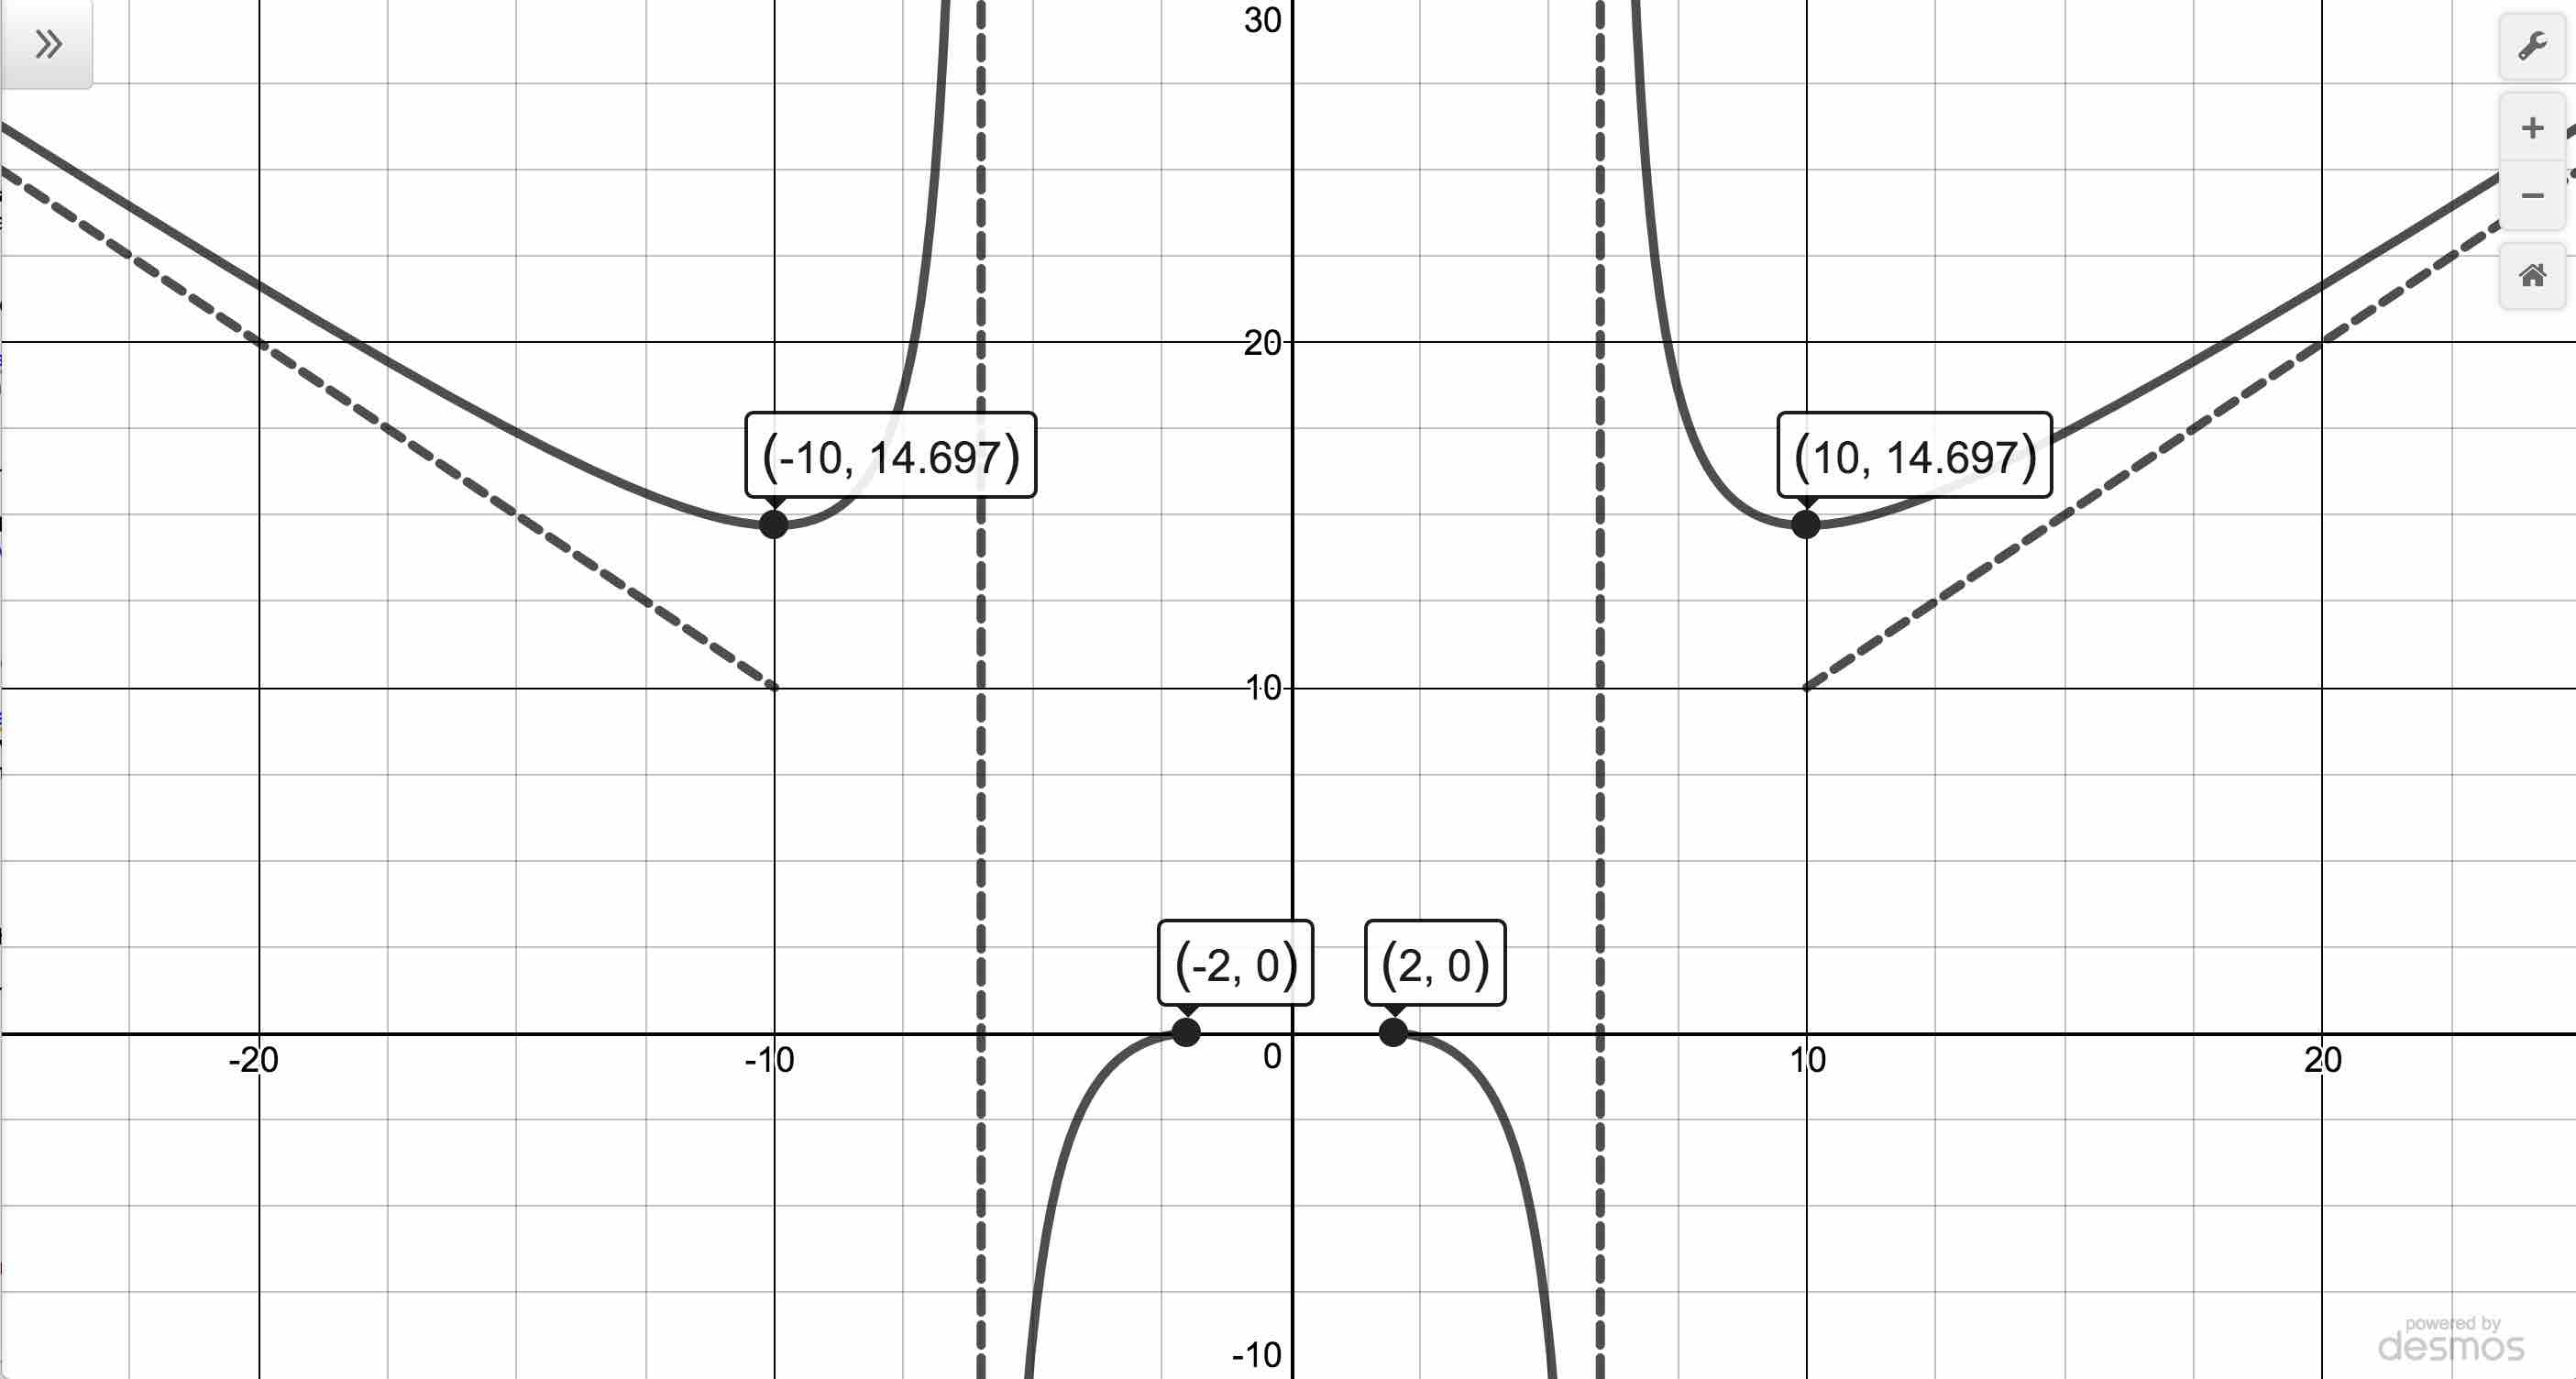
\includegraphics[width=3in]{./PowerFunctionsGraphics/RationalExpEx02.jpg} & 
 
\begin{mfpic}[20][10]{-2}{7}{-1.5}{1.5}
\arrow \polyline{(2,0), (-2,0)}
\arrow \polyline{(3,0), (7,0)}
\xmarks{0, 2, 3, 5}
\tlabel[cc](-1,1){$(+)$}
\tlabel[cc](0,-1){$-6 \hspace{7pt}$}
\tlabel[cc](0,1){\textinterrobang}
\tlabel[cc](1,1){$(-)$}
\tlabel[cc](2,-1){$-2 \hspace{7pt}$}
\tlabel[cc](2,1){$0$}
\tlabel[cc](3,-1){$2$}
\tlabel[cc](3,1){$0$}
\tlabel[cc](4,1){$(-)$}
\tlabel[cc](5,-1){$6$}
\tlabel[cc](5,1){\textinterrobang}
\tlabel[cc](6,1){$(+)$}

\end{mfpic} \\

The graph of $y=g(t)$  \hspace{0.75in} &Sign Diagram for $g(t)$ \\

\end{tabular}

\end{center} 

\qed

\end{enumerate}

\end{ex}

\subsection{Real Number Exponents}

We wish now to extend the concept of `exponent' from rational to all real numbers which means we need to discuss how to interpret an irrational exponent.  Once again, the notions presented here are best discussed using the language of Calculus or Analysis, but we nevertheless do what we can with the notions we have.  

Consider  the wildly famous irrational number $\pi$.  The number $\pi$ is defined geometrically as the ratio of the circumference of a circle to that circle's diameter.\footnote{This works for each and every circle, by the way, regardless of how large or small the circle is!} The reason we use the \textit{symbol} `$\pi$' instead of any numerical expression is that $\pi$ is an irrational number, and, as such, its decimal representation neither terminates nor repeats.  Hence we \textit{approximate} $\pi$ as $\pi \approx 3.14$ or $\pi \approx 3.14159265$.  No matter how many digits we write, however, what we have is a \textit{rational number} approximation of $\pi$. 


The good news is we can approximate $\pi$ to any desired accuracy using rational numbers by taking enough digits, so while we'll never `reach' the \textit{exact} value of $\pi$ with rational numbers, we can get \textit{as close as we like} to $\pi$ using rational numbers.  That being said, we assume $\pi$ exists on the real number line, despite the fact the list of digits to pinpoint its location is, in some sense, infinite.

We take this tack  when defining the value of a number raised to an irrational exponent.  Consider, for instance, $2^{\pi}$.  We can compute $2^3 = 8$, $2^{3.1} = 2^{\frac{31}{10}} = \sqrt[10]{2^{31}} \approx 8.574 $, $2^{3.14} = 2^{\frac{314}{100}} = 2^{\frac{157}{50}} = \sqrt[50]{2^{157}} \approx 8.8512$, and so on, so one way to  \textit{define} $2^{\pi}$ as the unique real number we obtain  as the exponents `approach' $\pi$. 

It is with this understanding that we present the notion of a `power function,' as described in Definition   \ref{powerfunction}:  $f(x) = a x^p$ where $a$ and $p$ are nonzero real number parameters.  Here the exponent $p$ is open to any (nonzero) real number.  Because of how we define real number exponents, if $p$ is irrational, then $ x \geq 0$ to avoid having negatives under even-indexed roots as we go through the approximation process.\footnote{or $x > 0$ if $p$ is negative.} 

In general, real number exponents inherit their properties from rational number exponents.  For instance, Theorem \ref{exponentprops} also holds for all real number exponents and the graphs of power functions inherit their behavior from graphs of rational exponent functions.  More specifically, the graphs of functions of the form $f(x)= x^p$ where $p>0$ all contain the points $(0,0)$ and $(1,1)$.  Moreover, these functions are increasing and their graphs are  concave down if $0<p<1$ and concave up if $p>1$. 


\begin{center}

\begin{mfpic}[17]{-1}{9}{-1}{9}
\axes
\tlabel[cc](9, -0.5){\scriptsize $x$}
\tlabel[cc](0.5, 9){\scriptsize $y$}
\tlabel[cc](5,8){\scriptsize $p>1$, concave up}
\tlabel[cc](6,1.5){\scriptsize $0<p<1$, concave down}
\tlabel[cc](0.5, -0.5){\scriptsize $(0,0)$}
\tlabel[cc](1.75, 0.75){\scriptsize $(1,1)$}
\penwd{1.25pt}
\arrow  \parafcn{0, 3,0.1}{(t**2,t)}
\arrow  \parafcn{0, 3,0.1}{(t,t**2)}
\point[4pt]{(0,0), (1,1)}
\tcaption{\scriptsize $f(x) = x^p$ for varying values of $p$.}

\end{mfpic}

\end{center}

Theorem \ref{linearrationalpowergraphs}  generalizes to real number power functions, so, for instance to graph $F(x) = (x-2)^{\pi}$, one need only start with $y = x^{\pi}$ and shift horizontally two units to the right.  (See the Exercises.)  

We close this section with an application to economics.  According to the \href{http://www.census.gov/library/publications/2016/demo/p60-256.html }{\underline{US Census}}, Table 2, the share of money income (2014-2015) is given in the table below on the left. From these data, we can create a cumulative distribution, $y = L(x)$ called the \index{Lorenz Curve}\textbf{Lorenz Curve}.   

The number $L(x)$ gives the percentage of the total national income earned by the bottom $x$ percent of wage earners, ranked from lowest income to highest income.  Since the population here is separated into `quintiles,' each data point corresponds to $20 \%$ of the population.  So, for example, $L(20)$ is the percentage of money income earned by the lowest $20 \%$ of wage earners.  In this case, we see $L(20) = 3.1$.  The number  $L(40)$ is the percentage of the money income earned by the bottom $40 \%$ of wage earners - so this includes not only the money from the Second Quintile, but also the Lowest Quintile:  $L(40) = 8.2 + L(20) = 8.2 +  3.1 = 11.3$.  Likewise, $L(60)$ is the total income share of the bottom $60 \%$ of wage earners which includes the income from the Middle, Second, and Lowest Quintiles:  $L(60) = 14.3 + L(40) = 14.3 + (8.2+3.1) = 25.6$.  

Continuing in this manner, we get $L(80) = 48.8$ and $L(100) = 100$, which is what we would expect:  $100 \%$ of the income is earned by $100 \%$ of the population.  We summarize these findings below  on the right.

\smallskip

\begin{tabular}{cc}

$ \begin{array}{cc}

\text{\small Portion of Population} & \text{ \small Percent of Money Income} \\

\text{\small Lowest Quintile} & \text{\small  3.1} \\

\text{\small Second Quintile} &\text{\small   8.2}  \\

\text{\small Middle Quintile} &  \text{\small 14.3}  \\

\text{\small Fourth Quintile} &  \text{\small  23.2}  \\

\text{\small Highest Quintile} &   \text{\small 51.2 } \\

\end{array} $
&

$ \begin{array}{cc}

\text{\small percent wage earners, $x$} & \text{\small percent income, $L(x)$} \\

\text{\small  20} & \text{\small 3.1}\\

\text{\small 40}  & \text{\small 11.3}  \\

\text{\small 60}  & \text{\small 25.6}  \\

\text{\small 80 }&   \text{\small 48.8}  \\

\text{\small 100}  &  \text{\small 100}  \\

\end{array} $


\end{tabular}

\enlargethispage{1in}

\begin{ex} \label{LorenzEx}  $~$

\begin{enumerate}

\item Find power function to model the Lorenz Curve: $L(x) = ax^p$.  Comment on the goodness of fit.  

\item Find and interpret $L(90)$.

\end{enumerate}

{\bf Solution.}  

\begin{enumerate}

\item Using \href{https://www.desmos.com/}{\underline{desmos}}, we get $L(x) = 0.00027901x^{2.7738}$ with $R^2 = 0.993$, indicating a pretty good fit.  

\begin{center}

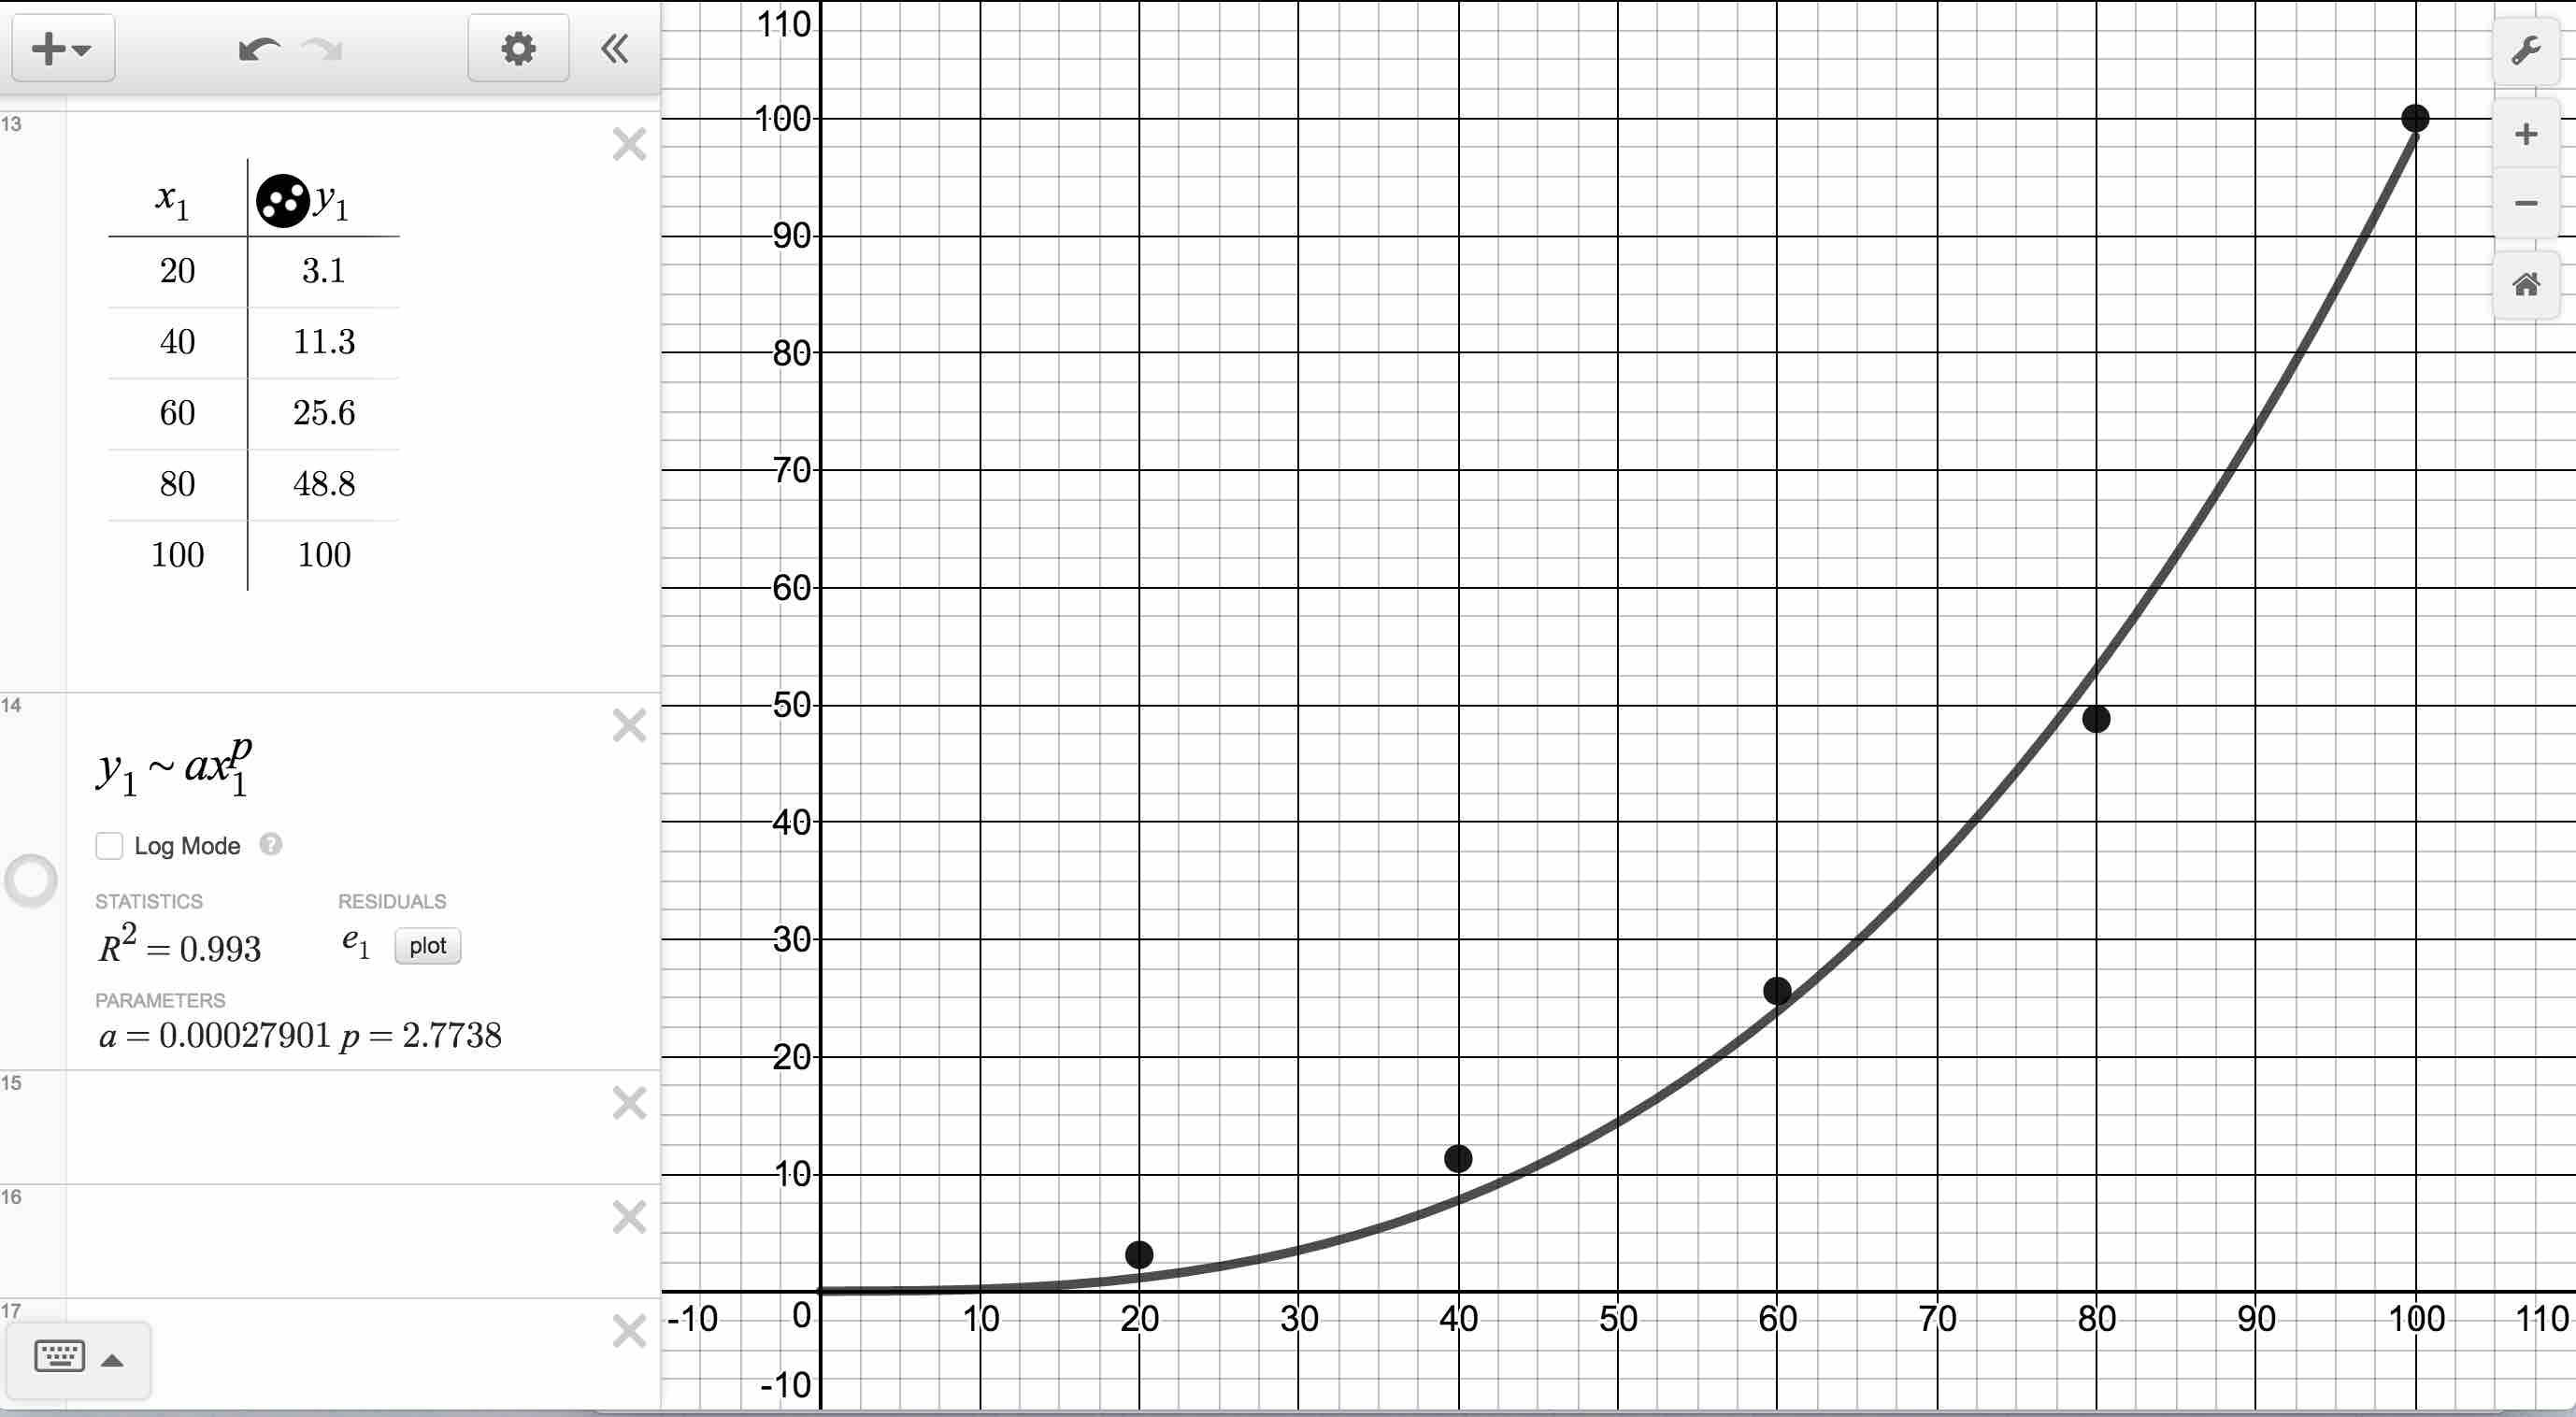
\includegraphics[width=3.5in]{./PowerFunctionsGraphics/LorenzEx.jpg}

\end{center}


\item We compute $L(90) = 0.00027901(90)^{2.7738} \approx 73.5$ meaning that the bottom $90 \%$ of the wage earners brought home $73.5 \%$ of the total income.  Said differently, the top $10 \%$ of wage earners made over $25 \%$ of the total national income.  \qed


\end{enumerate}


 
\end{ex}

\newpage

\subsection{Exercises}

In Exercises \ref{powergraphexfirst} - \ref{powergraphexlast}, use the given graphs along with Theorem \ref{linearrationalpowergraphs} to graph the given function.  Track at least two points and state the domain and range using interval notation.

\begin{center}

\begin{multicols}{2}

\begin{mfpic}[20]{-4}{4}{-1}{4}
\axes
\tlabel[cc](4, -0.5){\scriptsize $x$}
\tlabel[cc](0.5, 4){\scriptsize $y$}
\tlabel[cc](1.75,0.75){\scriptsize $(1,1)$}
\tlabel[cc](-1.75,0.75){\scriptsize $(-1,1)$}
\tlabel[cc](0.5,-0.5){\scriptsize $(0,0)$}
\penwd{1.25pt}
\arrow \reverse \arrow \parafcn{-1.5, 1.5,0.1}{(t**3,t**2)}
\point[4pt]{(-1,1), (0,0), (1,1)}
\tcaption{$f(x)=x^{\frac{2}{3}}$}
\end{mfpic}



\begin{mfpic}[20]{-4}{4}{-1}{4}
\axes
\tlabel[cc](4, -0.5){\scriptsize $t$}
\tlabel[cc](0.5, 4){\scriptsize $y$}
\tlabel[cc](2,1){\scriptsize $(1,1)$}
\tlabel[cc](0.5,-0.5){\scriptsize $(0,0)$}
\penwd{1.25pt}
\arrow  \function{0, 1.5,0.1}{x**3.14}
\point[4pt]{(0,0), (1,1)}
\tcaption{$g(t)=t^{\pi}$ \vphantom{{$f(x)=x^{\frac{2}{3}}$}}}
\end{mfpic}

\end{multicols}
\end{center}

\begin{multicols}{2}
\begin{enumerate}

\item $F(x) = (x-2)^{\frac{2}{3}}-1$ \label{powergraphexfirst}
\item $G(t) = (t+3)^{\pi} +1$

\setcounter{HW}{\value{enumi}}
\end{enumerate}
\end{multicols}

\begin{multicols}{2}
\begin{enumerate}
\setcounter{enumi}{\value{HW}}
\item $F(x) = 3-x^{\frac{2}{3}}$ 
\item $G(t) = (1-t)^{\pi}-2$  \vphantom{$F(x) = 3-x^{\frac{2}{3}}$ }

\setcounter{HW}{\value{enumi}}
\end{enumerate}
\end{multicols}


\begin{multicols}{2}
\begin{enumerate}
\setcounter{enumi}{\value{HW}}

\item $F(x) =(2x+5)^{\frac{2}{3}}+1$ \vphantom{$G(t) = \left( \dfrac{t+3}{2}\right)^{\pi}-1$}
\item $G(t) = \left( \dfrac{t+3}{2}\right)^{\pi}-1$ \label{powergraphexlast}
\setcounter{HW}{\value{enumi}}
\end{enumerate}
\end{multicols}

In Exercises \ref{findformulaforpowergraphfirst} - \ref{findformulaforpowergraphlast}, find a formula for each function below in the form $F(x) = a(bx-h)^{\frac{2}{3}}+k$.

\smallskip

\textbf{NOTE:}  There may be more than one solution!

\begin{multicols}{2}

\begin{enumerate}
\setcounter{enumi}{\value{HW}}

\item $~$ \label{findformulaforpowergraphfirst}  $y=F(x)$ %$F(x) = 2(x-1)^{\frac{2}{3}}-2$

\begin{mfpic}[20]{-4}{4}{-4}{4}
\axes
\tlabel[cc](4, -0.5){\scriptsize $x$}
\tlabel[cc](0.5, 4){\scriptsize $y$}
\tlabel[cc](1, -2.5){\scriptsize $(1,-2)$}
\tlabel[cc](2.5,-0.5){\scriptsize $(2,0)$}
\tlabel[cc](-0.5,-0.5){\scriptsize $(0,0)$}
\penwd{1.25pt}
\arrow \reverse \arrow \parafcn{-1.5, 1.5,0.1}{((t**3)+1,(2*(t**2))-2)}
\point[4pt]{(0,0), (1,-2), (2,0)}
\end{mfpic}
 



\item $~$ \label{findformulaforpowergraphlast} $y = F(x)$ %$F(x) =-(x+1)^{\frac{2}{3}} + 4$

\begin{mfpic}[10][20]{-10}{10}{-2}{6}
\axes
\tlabel[cc](10, -0.5){\scriptsize $x$}
\tlabel[cc](0.5, 6){\scriptsize $y$}
\tlabel[cc](-10, 0.5){\scriptsize $(-9,0)$}
\tlabel[cc](-1.5,4.5){\scriptsize $(-1,4)$}
\tlabel[cc](1.5,3){\scriptsize $(0,3)$}
\tlabel[cc](7,0.5){\scriptsize $(6,0)$}
\penwd{1.25pt}
\arrow \reverse \arrow \parafcn{-2.15,2.15 ,0.1}{((t**3)-1,4-(t**2))}
\point[4pt]{(-9,0), (7,0), (0,3), (-1,4)}
\end{mfpic}
 

\setcounter{HW}{\value{enumi}}

\end{enumerate}

\end{multicols}
\newpage

For each function in Exercises \ref{powerfcngraphexfirst} - \ref{powerfcngraphexlast} below 

\begin{itemize}

\item Analytically:

\begin{multicols}{3}

\begin{itemize}

\item find the domain.

\item find the axis intercepts.

\item analyze the end behavior.

\end{itemize}

\end{multicols}

\item Graph the function with help from a graphing utility and determine:

\begin{multicols}{2}

\begin{itemize}

\item  the range.

\item the local extrema, if they exist.

\end{itemize}

\end{multicols}

\begin{multicols}{2}

\begin{itemize}

\item intervals of increase/decrease.

\item any `unusual steepness' or `local' verticality.

\end{itemize}

\end{multicols}

\begin{multicols}{2}

\begin{itemize}

\item  vertical asymptotes.

\item  horizontal / slant asymptotes.

\end{itemize}

\end{multicols}

\item Construct a sign diagram for each function using the intercepts and graph.

\item  Comment on any observed symmetry.


\end{itemize}


\begin{multicols}{2}
\begin{enumerate}
\setcounter{enumi}{\value{HW}}

\item $f(x) = x^{\frac{2}{3}}(x - 7)^{\frac{1}{3}}$  \label{powerfcngraphexfirst}
\item $f(x) = x^{\frac{3}{2}}(x - 7)^{\frac{1}{3}}$ 


\setcounter{HW}{\value{enumi}}
\end{enumerate}
\end{multicols}

\begin{multicols}{2}
\begin{enumerate}
\setcounter{enumi}{\value{HW}}

\item $g(t) = 2t(t+3)^{-\frac{1}{3}}$ 
\item $g(t) = t^{\frac{3}{2}}(t-2)^{-\frac{1}{2}}$ 


\setcounter{HW}{\value{enumi}}
\end{enumerate}
\end{multicols}

\begin{multicols}{2}
\begin{enumerate}
\setcounter{enumi}{\value{HW}}

\item $f(x) = x^{0.4} (3-x)^{0.6}$ 
\item $f(x) = x^{0.5} (3-x)^{0.5}$ 


\setcounter{HW}{\value{enumi}}
\end{enumerate}
\end{multicols}

\begin{multicols}{2}
\begin{enumerate}
\setcounter{enumi}{\value{HW}}

\item $g(t) = 4t (9-t^2)^{-\sqrt{2}}$ 
\item $g(t) = 3(t^2+1)^{-\pi}$  \label{powerfcngraphexlast}


\setcounter{HW}{\value{enumi}}
\end{enumerate}
\end{multicols}

\begin{enumerate}
\setcounter{enumi}{\value{HW}}

\item \label{powerarcexercise}For each function $f(x)$ listed below, compute the average rate of change over the indicated interval.\footnote{See Definition \ref{arc} in Section \ref{AverageRateofChange} for a review of this concept, as needed.}  What trends do you observe?  How do your answers manifest themselves graphically?  Compare the results of this exercise with those of Exercise \ref{monomialarcexercise} in Section \ref{GraphsofPolynomials} and Exercise \ref{laurentarcexercise} in Section \ref{IntroRational}

\[ \begin{array}{|r||c|c|c|c|}  \hline

 f(x) &  [0.9, 1.1] & [0.99, 1.01] &[0.999, 1.001] & [0.9999, 1.0001]  \\ \hline
 x^{\frac{1}{2}} &&&&  \\  \hline
 x^{\frac{2}{3}} &&&&  \\ \hline
 x^{-0.23} &&&&   \\  \hline
 x^{\pi}  &&&&   \\  \hline

\end{array} \]

\item \label{WindChillTemperature} The \href{http://www.nws.noaa.gov/om/windchill/windchillglossary.shtml}{\underline{National Weather Service}} uses the following formula to calculate the wind chill: \[ W = 35.74 + 0.6215 \, T_{a} - 35.75\, V^{0.16} + 0.4275 \, T_{a} \, V^{0.16}  \] where $W$ is the wind chill temperature in $^{\circ}$F, $T_{a}$ is the air temperature in $^{\circ}$F, and  $V$ is the wind speed in miles per hour.  Note that $W$ is defined only for air temperatures at or lower than $50^{\circ}$F and wind speeds above $3$ miles per hour.

\begin{enumerate}

\item  Suppose the air temperature is $42^{\circ}$ and the wind speed is $7$ miles per hour. Find the wind chill temperature.  Round your answer to two decimal places.

\item  Suppose the air temperature is $37^{\circ}$F and the wind chill temperature is $30^{\circ}$F.  Find the wind speed.  Round your answer to two decimal places. 

\end{enumerate}

\item  As a follow-up to Exercise \ref{WindChillTemperature}, suppose the air temperature is $28^{\circ}$F.  

\begin{enumerate}

\item Use the formula from Exercise \ref{WindChillTemperature} to find an expression for the wind chill temperature as a function of the wind speed, $W(V)$.  

\item  \label{WindChill0} Solve $W(V) = 0$, round your answer to two decimal places,  and interpret.  

\item  Graph the function $W$ using a graphing utility and check your answer to part \ref{WindChill0}. 


\end{enumerate}


\item \label{pursuitfurther} Suppose Fritzy the Fox, positioned at a point $(x,y)$ in the first quadrant, spots Chewbacca the Bunny at $(0,0)$.   Chewbacca begins to run along a fence (the positive $y$-axis) towards his warren.  Fritzy, of course, takes chase and constantly adjusts his direction so that he is always running directly at Chewbacca.  If Chewbacca's speed is $v_{\mbox{\tiny$1$}}$ and  Fritzy's speed is $v_{\mbox{\tiny$2$}}$, the path Fritzy will take to intercept Chewbacca, provided $v_{\mbox{\tiny$2$}}$ is directly proportional to, but not equal to, $v_{\mbox{\tiny$1$}}$ is modeled by

\[ y = \dfrac{1}{2} \left(\dfrac{x^{1+ v_{1}/v_{2}}}{1+v_{\mbox{\tiny$1$}}/v_{\mbox{\tiny$2$}}}- \dfrac{x^{1-v_{\mbox{\tiny$1$}}/v_{\mbox{\tiny$2$}}}}{1-v_{\mbox{\tiny$1$}}/v_{\mbox{\tiny$2$}}}\right) + \dfrac{v_{\mbox{\tiny$1$}} v_{\mbox{\tiny$2$}}}{v_{\mbox{\tiny$2$}}^2-v_{\mbox{\tiny$1$}}^2} \]

\begin{enumerate}

\item  Determine the path that Fritzy will take if he runs exactly twice as fast as Chewbacca;  that is, $v_{\mbox{\tiny$2$}} = 2v_{\mbox{\tiny$1$}}$. Use your calculator to graph this path for $x \geq 0$.  What is the significance of the $y$-intercept of the graph?

\item  Determine the path Fritzy will take if Chewbacca runs exactly twice as fast as he does;  that is, $v_{\mbox{\tiny$1$}} = 2v_{\mbox{\tiny$2$}}$.  Use a graphing utility to graph this path for $x > 0$.  Describe the behavior of $y$ as $x \rightarrow 0^{+}$ and interpret this physically.

\item  With the help of your classmates, generalize parts (a) and (b) to two cases:  $v_{\mbox{\tiny$2$}} > v_{\mbox{\tiny$1$}}$ and $v_{\mbox{\tiny$2$}} < v_{\mbox{\tiny$1$}}$.   We will discuss the case of $v_{\mbox{\tiny$1$}} = v_{\mbox{\tiny$2$}}$ in Exercise \ref{pursuitlog} in Section \ref{ExpLogApplications}.

\end{enumerate}

\setcounter{HW}{\value{enumi}}
\end{enumerate}

\newpage

\subsection{Answers}

\begin{multicols}{2}
\begin{enumerate}

\item  $F(x) = (x-2)^{\frac{2}{3}}-1$ \\

\begin{mfpic}[20]{-2}{6}{-2}{3}
\axes
\tlabel[cc](6, -0.5){\scriptsize $x$}
\tlabel[cc](0.25, 3){\scriptsize $y$}
\tlabel[cc](3.5,-0.5){\scriptsize $(3,0)$}
\tlabel[cc](0.5,-0.5){\scriptsize $(1,0)$}
\tlabel[cc](2,-1.5){\scriptsize $(2,-1)$}
\penwd{1.25pt}
\arrow \reverse \arrow \parafcn{-1.5, 1.5,0.1}{(t**3+2,t**2-1)}
\point[4pt]{(1,0), (2,-1), (3,0)}
\tcaption{Domain:  $(-\infty, \infty)$, Range:  $[-1, \infty)$}
\end{mfpic}


\columnbreak


\item $G(t) = (t+3)^{\pi} +1$ \vphantom{$F(x) = (x-2)^{\frac{2}{3}}-1$}\\

\begin{mfpic}[20]{-7}{1}{0}{5}
\axes
\tlabel[cc](1, -0.5){\scriptsize $t$}
\tlabel[cc](0.5, 5){\scriptsize $y$}
\tlabel[cc](-1,2){\scriptsize $(-2,2)$}
\tlabel[cc](-2.5,0.5){\scriptsize $(-3,1)$}
\penwd{1.25pt}
\arrow  \function{-3,-1.5,0.1}{((x+3)**3.14)+1}
\point[4pt]{(-3,1), (-2,2)}
\tcaption{Domain:  $[-3, \infty)$, Range:  $[1, \infty)$}
\end{mfpic}


\setcounter{HW}{\value{enumi}}
\end{enumerate}
\end{multicols}

\begin{multicols}{2}
\begin{enumerate}
\setcounter{enumi}{\value{HW}}
\item  $F(x) = 3-x^{\frac{2}{3}} = (-1)x^{\frac{2}{3}} + 3$  \\

\begin{mfpic}[20]{-4}{4}{-1}{4}
\axes
\tlabel[cc](4, -0.5){\scriptsize $x$}
\tlabel[cc](0.5, 4){\scriptsize $y$}
\tlabel[cc](1.5,2.25){\scriptsize $(1,2)$}
\tlabel[cc](-1.75,2.25){\scriptsize $(-1,2)$}
\tlabel[cc](0.75,3){\scriptsize $(0,3)$}
\penwd{1.25pt}
\arrow \reverse \arrow \parafcn{-1.5, 1.5,0.1}{(t**3,3-(t**2))}
\point[4pt]{(-1,2), (0,3), (1,2)}
\tcaption{Domain: $(-\infty, \infty)$, Range: $(-\infty,3]$} 
\end{mfpic}


\columnbreak


\item  $G(t) = (1-t)^{\pi}-2 = ((-1)t+1)^{\pi}-2$  \vphantom{$F(x) = 3-x^{\frac{2}{3}}$} \\

\begin{mfpic}[20]{-4}{4}{-3}{2}
\axes
\tlabel[cc](4, -0.5){\scriptsize $t$}
\tlabel[cc](0.5, 2){\scriptsize $y$}
\tlabel[cc](2,-2){\scriptsize $(1,-2)$}
\tlabel[cc](0.75,-1){\scriptsize $(0,-1)$}
\penwd{1.25pt}
\arrow  \reverse \function{-0.5, 1,0.1}{((1-x)**3.14)-2}
\point[4pt]{(0,-1), (1,-2)}
\tcaption{Domain:  $(-\infty, 1]$, Range: $[-2, \infty)$}
\end{mfpic}

\setcounter{HW}{\value{enumi}}
\end{enumerate}
\end{multicols}

\begin{multicols}{2}
\begin{enumerate}
\setcounter{enumi}{\value{HW}}
\item  $F(x) =(2x+5)^{\frac{2}{3}}+1$ \vphantom{$G(t) = \left( \dfrac{t+3}{2}\right)^{\pi}-1$}  \\

\begin{mfpic}[20]{-6.5}{1.5}{-1}{4}
\axes
\tlabel[cc](1.5, -0.5){\scriptsize $x$}
\tlabel[cc](0.5, 4){\scriptsize $y$}
\tlabel[cc](-4,1.75){\scriptsize $(-3,2)$}
\tlabel[cc](-2.5,0.5){\scriptsize $\left(-\frac{5}{2},1 \right)$}
\tlabel[cc](-1,1.75){\scriptsize $(-2,2)$}
\penwd{1.25pt}
\arrow \reverse \arrow \parafcn{-1.6, 1.6,0.1}{( 0.5*( (t**3)-5),(t**2)+1)}
\point[4pt]{(-3,2), (-2.5,1), (-2,2)}
\tcaption{Domain: $(-\infty, \infty)$, Range: $[1, \infty)$}
\end{mfpic}


\columnbreak


\item  $G(t) = \left( \dfrac{t+3}{2}\right)^{\pi}-1= \left( \frac{1}{2} \, t + \frac{3}{2}\right)^{\pi} -1$\\

\begin{mfpic}[20]{-4}{4}{-2}{3}
\axes
\tlabel[cc](4, -0.5){\scriptsize $t$}
\tlabel[cc](0.5, 3){\scriptsize $y$}
\tlabel[cc](-3,-1.5){\scriptsize $(-3,-1)$}
\tlabel[cc](-1.5,0.5){\scriptsize $(-1,0)$}
\penwd{1.25pt}
\arrow  \function{-3, -0.2,0.1}{(((x+3)/2)**3.14)-1}
\point[4pt]{(-3,-1), (-1,0)}
\tcaption{Domain:  $[-3, \infty)$, Range: $[-1, \infty)$}
\end{mfpic}

\setcounter{HW}{\value{enumi}}
\end{enumerate}
\end{multicols}

\begin{multicols}{2}

\begin{enumerate}
\setcounter{enumi}{\value{HW}}

\item One solution is: $F(x) = 2(x-1)^{\frac{2}{3}}-2$

\item  One solution is: $F(x) =-(x+1)^{\frac{2}{3}} + 4$


\setcounter{HW}{\value{enumi}}
\end{enumerate}

\end{multicols}

\newpage

\begin{enumerate}
\setcounter{enumi}{\value{HW}}

\item \begin{multicols}{2} 
$f(x) = x^{\frac{2}{3}}(x - 7)^{\frac{1}{3}}$\\
Domain: $(-\infty, \infty)$\\
Intercepts: $(0,0)$, $(7,0)$\\
Graph: \\

\begin{mfpic}[10]{-4}{10}{-5}{5.5}
\axes
\tlabel[cc](10,-0.5){\scriptsize $x$}
\tlabel[cc](0.5,5.5){\scriptsize $y$}
\tlabel[cc](5,-5){\scriptsize $\approx (4.667, -3.704)$}
\xmarks{-3 step 1 until 9}
\ymarks{-4 step 1 until 5}
\tlpointsep{4pt}
\tiny
\axislabels {x}{{$-3 \hspace{6pt}$} -3, {$-2 \hspace{6pt}$} -2, {$-1 \hspace{6pt}$} -1, {$1$} 1, {$2$} 2, {$3$} 3, {$4$} 4, {$5$} 5, {$6$} 6,  {$8$} 8, {$9$} 9}
\axislabels {y}{{$-4$} -4, {$-3$} -3, {$-2$} -2,  {$1$} 1, {$2$} 2, {$3$} 3, {$4$} 4, {$5$} 5}
\normalsize
\point[4pt]{(0,0), (7,0), (4.667, -3.704)}
\dashed \polyline{(-3, -5.33), (9, 6.67)}
\penwd{1.25pt}
\arrow \reverse \function{-3,0,0.1}{-((x**2)**(1/3))*((7 - x)**(1/3))}
\function{0,7,0.1}{-((x**2)**(1/3))*((7 - x)**(1/3))}
\arrow \function{7,9,0.1}{((x**2)**(1/3))*((x - 7)**(1/3))}
\end{mfpic}

\vfill
\columnbreak

As $x \rightarrow -\infty$, $f(x) \rightarrow -\infty$\\
As $x \rightarrow \infty$, $f(x) \rightarrow \infty$\\
Range: $(-\infty, \infty)$\\
Local minimum: $\approx (4.667, -3.704)$\\
Local maximum: $(0,0)$ (this is a cusp) \\
Increasing: $(-\infty, 0]$, $\approx [4.667, \infty)$\\
Decreasing: $[0, 4.667]$\\
Unusual steepness at $x = 7$\\
Using Calculus it can be shown that $y = x - \frac{7}{3}$ is a slant asymptote of this graph.\\
Sign Diagram:\\

\smallskip

\begin{mfpic}[10]{-3}{10}{-2}{2}
\arrow \reverse \arrow \polyline{(-3,0),(10,0)}
\xmarks{0,7}
\tlabel[cc](-1.5,1){$(-)$}
\tlabel[cc](0,-1){$0$}
\tlabel[cc](0,1){$0$}
\tlabel[cc](3.5,1){$(-)$}
\tlabel[cc](7,-1){$7$}
\tlabel[cc](7,1){$0$}
\tlabel[cc](8.5,1){$(+)$}
\end{mfpic}



\end{multicols}

\item \begin{multicols}{2} 
$f(x) = x^{\frac{3}{2}}(x - 7)^{\frac{1}{3}}$\\
Graph: \\
\begin{mfpic}[15][3]{-1}{8.5}{-20}{30}
\axes
\tlabel[cc](8.5,-3){\scriptsize $x$}
\tlabel[cc](0.5,30){\scriptsize $y$}
\tlabel[cc](6,-18){\scriptsize $\approx (5.727, -14.854)$}
\xmarks{1 step 1 until 8}
\ymarks{-15 step 5 until 25}
\tlpointsep{4pt}
\scriptsize
\axislabels {x}{ {$2$} 2, {$3$} 3, {$4$} 4, {$5$} 5, {$6$} 6,  {$8$} 8}
\axislabels {y}{{$-15$} -15, {$-10$} -10, {$-5$} -5, {$5$} 5, {$10$} 10, {$15$} 15, {$20$} 20, {$25$} 25}
\normalsize
\point[4pt]{(0,0), (7,0), (5.727, -14.854)}
\penwd{1.25pt}
\function{0,7,0.1}{-(x**1.5)*((7 - x)**(1/3))}
\arrow \function{7,8.5,0.1}{(x**1.5)*((x - 7)**(1/3))}
\end{mfpic}


\vfill
\columnbreak

Domain: $[0, \infty)$\\
Intercepts: $(0,0)$, $(7,0)$\\
As $x \rightarrow \infty$, $f(x) \rightarrow \infty$\\
Range:  $\approx [-14.854, \infty)$\\
Local minimum:  $\approx (5.727, -14.854)$\\
Increasing: $\approx [5.727, \infty)$\\
Decreasing: $\approx [0, 5.727]$\\
Unusual steepness at $x = 7$\\
Sign Diagram:\\

\smallskip

\begin{mfpic}[15]{0}{10}{-1}{1}
\reverse \arrow \polyline{(0,0),(10,0)}
\xmarks{0, 7}
\tlabel[cc](0,-0.5){$0$}
\tlabel[cc](0,0.5){$0$}
\tlabel[cc](3.5, 0.5){$(-)$}
\tlabel[cc](7,-0.5){$7$}
\tlabel[cc](7,0.5){$0$}
\tlabel[cc](8, 0.5){$(+)$}
\end{mfpic}


\end{multicols}

\setcounter{HW}{\value{enumi}}
\end{enumerate}


\begin{enumerate}
\setcounter{enumi}{\value{HW}}

\item \begin{multicols}{2} 
 $g(t) = 2t(t+3)^{-\frac{1}{3}}$ \\
Graph: \\

\begin{mfpic}[10][5]{-10}{5}{-10}{10}
\axes
\tlabel[cc](5,-0.5){\scriptsize $t$}
\tlabel[cc](0.5,10){\scriptsize $y$}
\tlabel[cc](-6,5){\scriptsize $\approx (-4.5, 7.862)$}
\xmarks{-9 step 1 until 4}
\ymarks{-8 step 2 until 8}
\tlpointsep{4pt}
\tiny
\axislabels {x}{{$-9 \hspace{6pt}$} -9, {$-8 \hspace{6pt}$} -8, {$-7 \hspace{6pt}$} -7, {$-6 \hspace{6pt}$} -6, {$-5 \hspace{6pt}$} -5, {$-4 \hspace{6pt}$} -4, {$-3 \hspace{6pt}$} -3, {$-2 \hspace{6pt}$} -2, {$-1 \hspace{6pt}$} -1, {$1$} 1, {$2$} 2, {$3$} 3, {$4$} 4}
\axislabels {y}{ {$-8$} -8,  {$-6$} -6, {$-4$} -4, {$-2$} -2,   {$2$} 2, {$4$} 4,  {$6$} 6,  {$8$} 8}
\normalsize
\dashed \polyline{(-3,-9), (-3, 10)}
\point[4pt]{(0,0), (-4.5, 7.862)}
\penwd{1.25pt}
\arrow \reverse \arrow \function{-9,-3.2,0.1}{-(2*x)/((-x-3)**(1/3))}
\arrow \reverse \function{-2.8,0,0.1}{(2*x)/((x+3)**(1/3))}
\arrow \function{0,5,0.1}{(2*x)/((x+3)**(1/3))}

\end{mfpic}

\vfill
\columnbreak

Domain: $(-\infty, -3) \cup (-3, \infty)$\\
Intercept: $(0,0)$\\
As $t \rightarrow \pm \infty$, $g(t) \rightarrow \infty$\\
Range: $(-\infty, \infty)$\\
Local minimum: $\approx (-4.5, 7.862)$\\
Increasing: $\approx [-4.5, -3)$, $(-3,\infty)$ \\
Decreasing: $\approx (-\infty, -4.5]$\\
Vertical Asymptote:  $t = -3$\\
Sign Diagram:\\

\smallskip

\begin{mfpic}[10]{-3}{10}{-2}{2}
\arrow \reverse \arrow \polyline{(-3,0),(10,0)}
\xmarks{0,7}
\tlabel[cc](-1.5,1){$(+)$}
\tlabel[cc](0,-1){$-3 \hspace{6pt}$}
\tlabel[cc](0,1){\textinterrobang}
\tlabel[cc](3.5,1){$(-)$}
\tlabel[cc](7,-1){$0$}
\tlabel[cc](7,1){$0$}
\tlabel[cc](8.5,1){$(+)$}
\end{mfpic}



\end{multicols}

\item \begin{multicols}{2} 
$g(t)= t^{\frac{3}{2}}(t-2)^{-\frac{1}{2}}$\\
Domain:  $(2, \infty)$\\
As $t \rightarrow \infty$, $g(t) \rightarrow \infty$\\
Graph: \\
\begin{mfpic}[15][10]{-1}{10}{-1}{10}
\axes
\tlabel[cc](10,-0.5){\scriptsize $t$}
\tlabel[cc](0.5,10){\scriptsize $y$}
\xmarks{1 step 1 until 9}
\ymarks{1 step 2 until 9}
\tlpointsep{4pt}
\tiny
\axislabels {x}{{$1$} 1, {$2$} 2, {$3$} 3, {$4$} 4, {$5$} 5, {$6$} 6,  {$7$} 7, {$8$} 8, {$9$} 9}
\axislabels {y}{{$1$} 1,  {$3$} 3, {$5$} 5,  {$7$} 7,  {$9$} 9}
\normalsize
\dashed \polyline{(2,5), (2,9)}
\dashed \polyline{(4,5), (9,10)}
\gclear \tlabelrect(3,4){\scriptsize $\approx (3, 5.196)$}
\point[4pt]{(3, 5.196)}
\penwd{1.25pt}
\arrow \reverse \arrow \function{2.1,8.75,0.1}{(x**1.5)*((x - 2)**(-0.5))}
\end{mfpic}


\vfill
\columnbreak

Range:  $\approx [5.196, \infty)$\\
Local minimum:  $\approx (3, 5.196)$\\
Increasing: $\approx [3, \infty)$\\
Decreasing: $\approx (2,3]$\\
Vertical asymptote:  $t = 2$\\
Using Calculus it can be shown that $y = t+1$ is a slant asymptote of this graph.\\
Sign Diagram:\\

\smallskip

\begin{mfpic}[15]{0}{10}{-1}{1}
\reverse \arrow \polyline{(0,0),(4,0)}
\xmarks{0}
\tlabel[cc](0,-0.5){$2$}
\tlabel[cc](0,0.5){\textinterrobang}
\tlabel[cc](2, 0.5){$(+)$}
\end{mfpic}


\end{multicols}

\setcounter{HW}{\value{enumi}}
\end{enumerate}



\begin{enumerate}
\setcounter{enumi}{\value{HW}}

\item \begin{multicols}{2} 
 $f(x) = x^{0.4}(3-x)^{0.6}$ \\
 Domain: $(-\infty,  \infty)$\\
Intercepts: $(0,0)$, $(3,0)$\\
Graph: \\
\begin{mfpic}[20]{-2}{5}{-2}{4}
\axes
\tlabel[cc](5,-0.5){\scriptsize $x$}
\tlabel[cc](0.5,4){\scriptsize $y$}
\tlabel[cc](2,2){\scriptsize $\approx (1.2, 1.531)$}
\xmarks{-1 step 1 until 4}
\ymarks{-1 step 1 until 3}
\tlpointsep{4pt}
\tiny
\axislabels {x}{ {$-1 \hspace{6pt}$} -1, {$1$} 1, {$2$} 2,  {$4$} 4}
\axislabels {y}{{$-1$} -1,   {$2$} 2,   {$3$} 3,   {$4$} 4}
\normalsize
%\dashed \polyline{(-3,-9), (-3, 10)}
\point[4pt]{(0,0), (3,0), (1.2, 1.531)}
\penwd{1.25pt}
\arrow \reverse \function{-2,0,0.1}{((-x)**0.4)*((3-x)**0.6)}
\function{0,3,0.1}{(x**0.4)*((3-x)**0.6)}
\arrow \function{3,4,0.1}{-(x**0.4)*((x-3)**0.6)}

\end{mfpic}

\vfill
\columnbreak


As $x \rightarrow -\infty$, $f(x) \rightarrow \infty$\\
As $x \rightarrow \infty$, $f(x) \rightarrow -\infty$\\
Range: $(-\infty, \infty)$\\
Local minimum: $(0,0)$ (this is a cusp)\\
Local maximum: $\approx (1.2, 1.531)$\\
Increasing: $\approx [0, 1.2]$ \\
Decreasing: $\approx (-\infty, 0]$, $[1.2, \infty)$\\
Unusual Steepness:  $x = 3$\\
Sign Diagram:\\

\smallskip

\begin{mfpic}[10]{-3}{10}{-2}{2}
\arrow \reverse \arrow \polyline{(-3,0),(10,0)}
\xmarks{0,7}
\tlabel[cc](-1.5,1){$(+)$}
\tlabel[cc](0,-1){$0$}
\tlabel[cc](0,1){$0$}
\tlabel[cc](3.5,1){$(+)$}
\tlabel[cc](7,-1){$3$}
\tlabel[cc](7,1){$0$}
\tlabel[cc](8.5,1){$(-)$}
\end{mfpic}



\end{multicols}

\item \begin{multicols}{2} 
 $f(x) = x^{0.5}(3-x)^{0.5}$ \\
Graph: \\
\begin{mfpic}[20]{-2}{5}{-2}{4}
\axes
\tlabel[cc](5,-0.5){\scriptsize $x$}
\tlabel[cc](0.5,4){\scriptsize $y$}
\tlabel[cc](2,2){\scriptsize $\approx (1.5, 1.5)$}
\xmarks{-1 step 1 until 4}
\ymarks{-1 step 1 until 3}
\tlpointsep{4pt}
\tiny
\axislabels {x}{ {$-1 \hspace{6pt}$} -1, {$1$} 1, {$2$} 2,  {$4$} 4}
\axislabels {y}{{$-1$} -1,   {$1$} 1,  {$2$} 2,   {$3$} 3}
\normalsize
\point[4pt]{(0,0), (3,0), (1.5, 1.5)}
\penwd{1.25pt}
\function{0,3,0.1}{(x**0.5)*((3-x)**0.5)}
\end{mfpic}

\vfill
\columnbreak

Domain: $[0,3]$\\
Intercepts: $(0,0)$, $(3,0)$\\
Range: $\approx [0, 1.5]$\\
Increasing: $\approx [0, 1.5]$ \\
Decreasing: $\approx [1.5, 3]$\\
Unusual Steepness:\footnote{Note you may need to zoom in to see this.}  $x=0$, $x = 3$\\
Sign Diagram:\\

\smallskip

\begin{mfpic}[10]{-3}{10}{-2}{2}
 \polyline{(0,0),(7,0)}
\xmarks{0,7}
\tlabel[cc](0,-1){$0$}
\tlabel[cc](0,1){$0$}
\tlabel[cc](3.5,1){$(+)$}
\tlabel[cc](7,-1){$3$}
\tlabel[cc](7,1){$0$}
\end{mfpic}
\end{multicols}
\setcounter{HW}{\value{enumi}}
\end{enumerate}

\newpage

\begin{enumerate}
\setcounter{enumi}{\value{HW}}

\item \begin{multicols}{2} 
$g(t) = 4t (9-t^2)^{-\sqrt{2}}$\\
Graph: \\
\begin{mfpic}[15]{-4}{4}{-3}{3}
\axes
\tlabel[cc](4,-0.5){\scriptsize $t$}
\tlabel[cc](0.5,4){\scriptsize $y$}
\xmarks{-2 step 1 until 2}
\ymarks{-2 step 1 until 2}
\tlpointsep{4pt}
\tiny
\axislabels {x}{ {$-2 \hspace{6pt}$} -2,{$-1 \hspace{6pt}$} -1, {$1$} 1, {$2$} 2}
\axislabels {y}{{$-2$} -2, {$-1$} -1,   {$1$} 1,   {$2$} 2}
\normalsize
\dashed \polyline{(-3,-3), (-3, 3)}
\dashed \polyline{(3,-3), (3, 3)}
\point[4pt]{(0,0)}
\penwd{1.25pt}
\arrow \reverse \arrow  \function{-2.6,2.6,0.1}{4*x/((9-(x**2))**1.414)}
\end{mfpic}

\vfill
\columnbreak
 Domain: $(-3, 3)$\\
Intercepts: $(0,0)$\\
Range: $(-\infty, \infty)$\\
Increasing: $(-3,3)$ \\
Sign Diagram:\\

\smallskip

\begin{mfpic}[10]{-5}{5}{-2}{2}
\polyline{(-5,0),(5,0)}
\xmarks{-5,0,5}
\tlabel[cc](-5,-1){$-3 \hspace{6pt}$}
\tlabel[cc](-5,1){\textinterrobang}
\tlabel[cc](-2.5,1){$(-)$}
\tlabel[cc](0,-1){$0$}
\tlabel[cc](0,1){$0$}
\tlabel[cc](2.5,1){$(+)$}
\tlabel[cc](5,-1){$3$}
\tlabel[cc](5,1){\textinterrobang}
\end{mfpic}

Note:  $g$ is odd

\end{multicols}

\item \begin{multicols}{2} 
$g(t) = 3(t^2+1)^{-\pi}$ \\
Domain: $(-\infty, \infty)$\\
Graph: \\
\begin{mfpic}[20]{-4}{4}{-1}{4}
\axes
\tlabel[cc](4,-0.5){\scriptsize $t$}
\tlabel[cc](0.5,4){\scriptsize $y$}
\xmarks{-3 step 1 until 3}
\ymarks{1 step 1 until 3}
\tlpointsep{4pt}
\tiny
\axislabels {x}{ {$-3 \hspace{6pt}$} -3,{$-2 \hspace{6pt}$} -2,{$-1 \hspace{6pt}$} -1, {$1$} 1, {$2$} 2, {$3$} 3}
\axislabels {y}{ {$1$} 1,   {$2$} 2,   {$3$} 3}
\normalsize
\point[4pt]{(0,3)}
\penwd{1.25pt}
\arrow \reverse \arrow  \function{-3,3,0.1}{3/(((x**2)+1)**3.14)}
\end{mfpic}

\vfill
\columnbreak

Intercept: $(0,3)$\\
As $t \rightarrow \pm \infty$, $g(t) \rightarrow 0$ \\
Range: $(0, 3]$\\
Increasing: $(-\infty, 0]$ \\
Decreasing: $[0, \infty)$\\
Horizontal asymptote:  $y =0$\\
Sign Diagram:\\

\vspace*{-0.2in}

\begin{mfpic}[10]{-5}{5}{-2}{2}
 \arrow \reverse \arrow \polyline{(-5,0),(5,0)}

\tlabel[cc](0,1){$(+)$}

\end{mfpic}

Note:  $g$ is even

\end{multicols}
\setcounter{HW}{\value{enumi}}
\end{enumerate}

\begin{enumerate}
\setcounter{enumi}{\value{HW}}

\item As in  Exercise \ref{monomialarcexercise} in Section \ref{GraphsofPolynomials} and Exercise \ref{laurentarcexercise} in Section \ref{IntroRational}, the slopes of these curves near $x = 1$ approach the value of the exponent on $x$.

\[ \begin{array}{|r||c|c|c|c|}  \hline

 f(x) &  [0.9, 1.1] & [0.99, 1.01] &[0.999, 1.001] & [0.9999, 1.0001]  \\ \hline
 x^{\frac{1}{2}} & 0.5006 & \approx \frac{1}{2} & \approx \frac{1}{2} & \approx \frac{1}{2} \\ [5pt] \hline
 x^{\frac{2}{3}} & 0.6672 & 0.6667 & \approx \frac{2}{3} & \approx \frac{2}{3}  \\ [5pt] \hline
 x^{-0.23} & -0.2310 & \approx -0.23 &\approx -0.23 &  \approx -0.23  \\  \hline
 x^{\pi}  &3.1544 & 3.1417 & \approx \pi & \approx \pi   \\  \hline

\end{array} \]

\item

\begin{enumerate}

\item  $W \approx 37.55^{\circ}$F.

\item  $V \approx 9.84$ miles per hour.

\end{enumerate}

\item 

\begin{enumerate}

\item $W(V) = 53.142 - 23.78 V^{0.16}$.  Since we are told in Exercise \ref{WindChillTemperature} that wind chill is only effect for wind speeds of more than 3 miles per hour, we restrict the domain to $V > 3$.

\item $W(V)=0$ when $V \approx 152.29$.  This means, according to the model, for the wind chill temperature to be $0^{\circ}$F, the wind speed needs to be $152.29$ miles per hour.

\newpage

\item The graph of $y = W(V)$ is below.  \\

\centerline{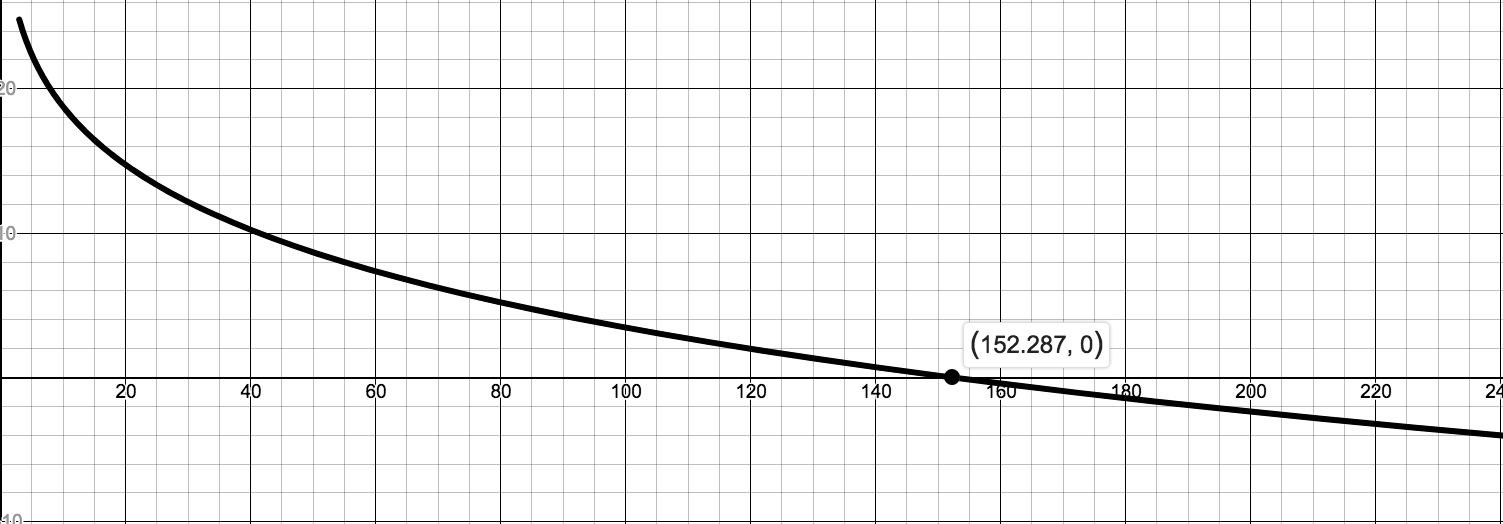
\includegraphics[height=1.75in]{./PowerFunctionsGraphics/WINDCHILL.jpg}}

\end{enumerate}



\item \begin{enumerate}

\item  $y = \frac{1}{3}x^{\frac{3}{2}} - x^{\frac{1}{2}} + \frac{2}{3}$.  The point $\left(0,\frac{2}{3}\right)$ is when Fritzy's path crosses Chewbacca's path - in other words, where Fritzy catches Chewbacca.

\begin{center} 

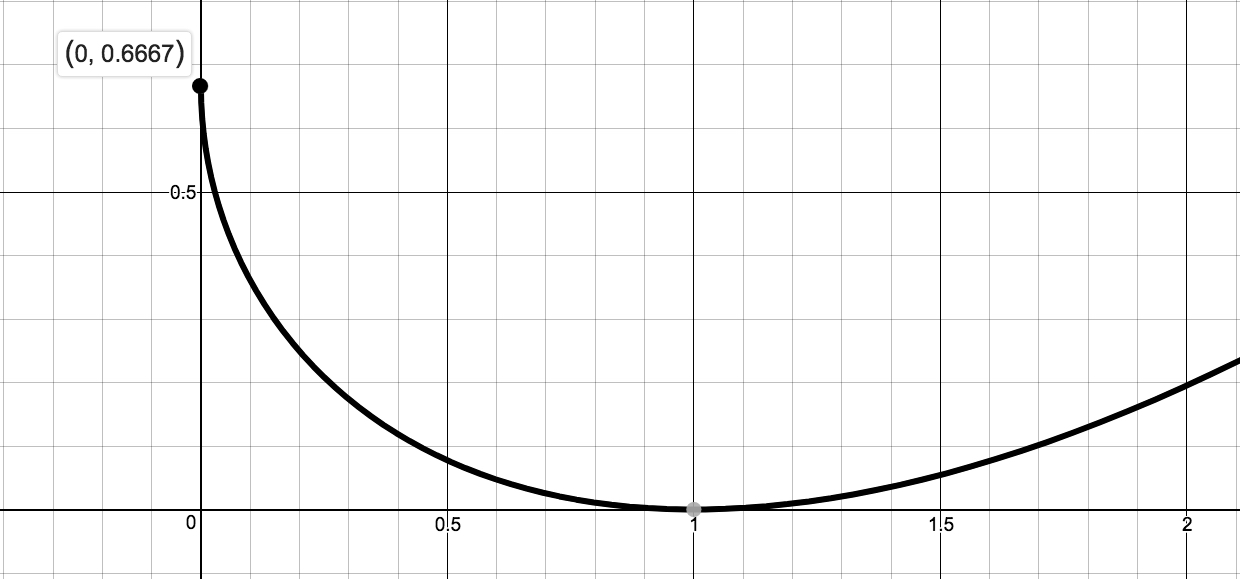
\includegraphics[height=2in]{./PowerFunctionsGraphics/PURSUIT01.jpg}

 $y = \frac{1}{3}x^{\frac{3}{2}} - x^{\frac{1}{2}} + \frac{2}{3}$

\end{center}

\item $y = \frac{1}{6}x^3+\frac{1}{2}x^{-1} - \frac{2}{3}$.  We find as $x \rightarrow 0^{+}$, $y \rightarrow \infty$ which means, in this case, Fritzy's pursuit never ends;  he never catches Chewbacca. This makes sense since Chewbacca has a head start and is running faster than Fritzy.

\begin{center} 

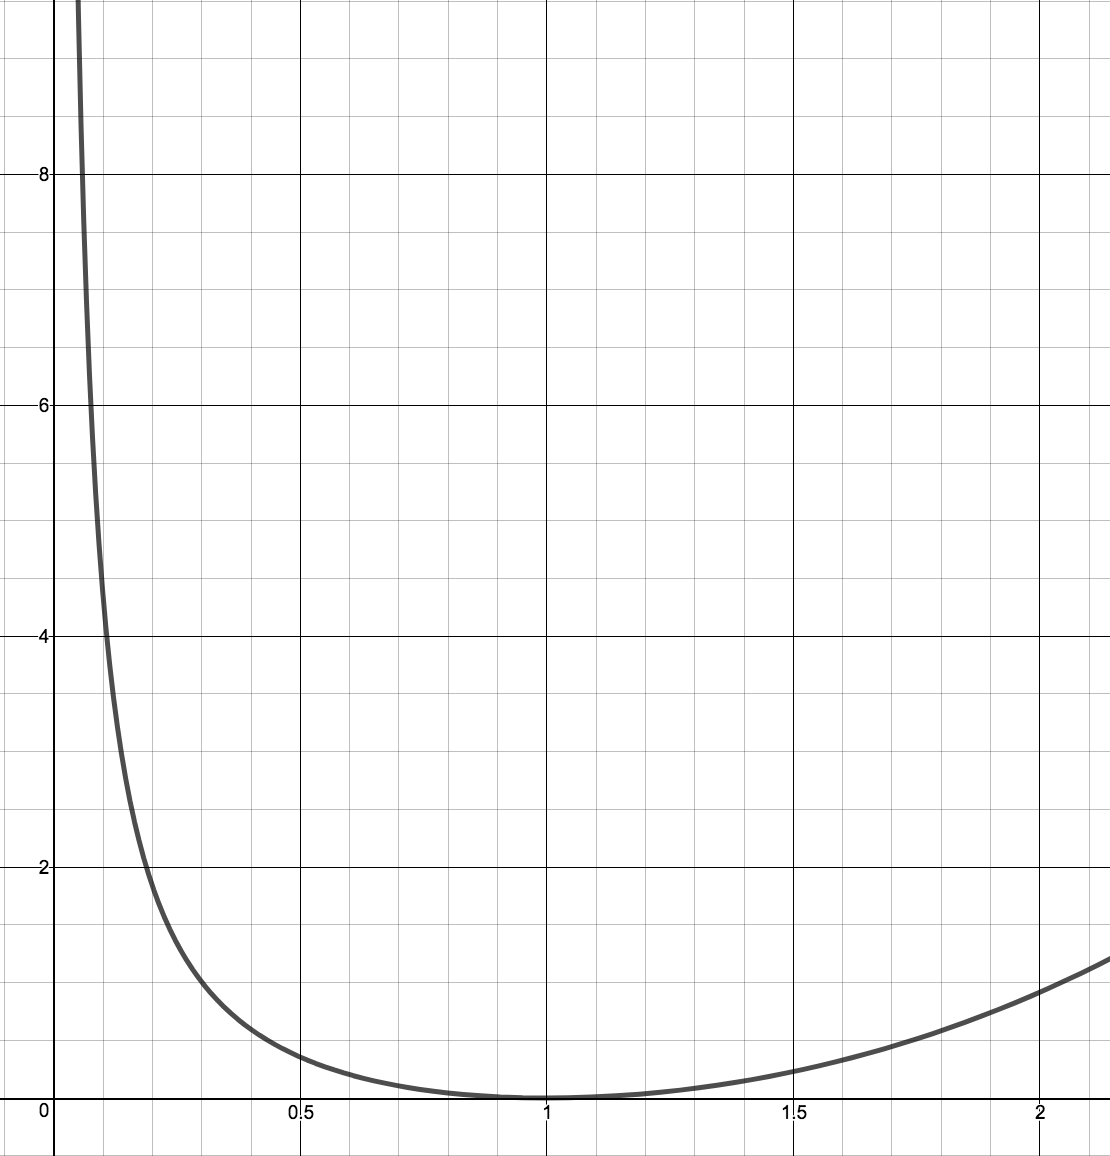
\includegraphics[height=2in]{./PowerFunctionsGraphics/PURSUIT02.jpg}

 $y = \frac{1}{6}x^3+\frac{1}{2}x^{-1} - \frac{2}{3}$

\end{center}


\end{enumerate}






\setcounter{HW}{\value{enumi}}
\end{enumerate}




\closegraphsfile